%-------------------------------------------------------------------------------
%                      Template Naskah Skripsi
%               	Berdasarkan format JTETI FT UGM
% 						(c) @gunturdputra 2014
%-------------------------------------------------------------------------------

%Template pembuatan naskah skripsi.
\documentclass{jtetiskripsi}

%Untuk prefiks pada daftar gambar dan tabel
\usepackage[titles]{tocloft}
\renewcommand\cftfigpresnum{Gambar\  }
\renewcommand\cfttabpresnum{Tabel\   }

%Untuk hyperlink dan table of content
\usepackage{hyperref}
\newlength{\mylenf}
\settowidth{\mylenf}{\cftfigpresnum}
\setlength{\cftfignumwidth}{\dimexpr\mylenf+2em}
\setlength{\cfttabnumwidth}{\dimexpr\mylenf+2em}

%Untuk Bold Face pada Keterangan Gambar
\usepackage[labelfont=bf]{caption}

%Untuk caption dan subcaption
\usepackage{caption}
\usepackage{subcaption}

%pdf
\usepackage{pdfpages}

%table
\usepackage{graphics}

\usepackage{wrapfig}

%-----------------------------------------------------------------
%Disini awal masukan untuk data proposal skripsi
%-----------------------------------------------------------------
\titleind{Implementasi Steganografi dalam Penyembunyian Pesan pada Citra Digital dengan Metode \emph{Least Significant Bit}}

\fullname{AMELIA APRILIANI}

\idnum{3145143626}

\approvaldate{02 Februari 2017}

\degree{Sarjana Ilmu Komputer}

\yearsubmit{2018}

\program{Ilmu Komputer}

\dept{Ilmu Komputer}

\firstsupervisor{Drs. Mulyono, M.Kom.}
\firstnip{1196605171994031003}

\secondsupervisor{Ratna Widyati, S.Si, M.Kom.}
\secondnip{197509252002122002}

%hypenation

\hyphenation{eng-gan me-ngem-bang-kan smart-phone bah-kan You-Tube you-tube di-lan-jut-kan pe-rang-kat di-la-ku-kan di-mung-kin-kan mem-pro-ses me-mung-kin-kan pe-ra-la-tan plat-form You-Tube-An-dro-id-Pla-yer-A-pi me-nge-ta-hu-i me-mu-dah-kan ba-han se-dang-kan con-trol-ler meng-u-bah me-nam-bah-kan App-Com-pat-Ac-ti-vi-ty pe-ring-kat di-se-su-ai-kan di-bu-tuh-kan pe-rin-tah me-nge-lo-la pe-nge-lo-la-an ber-a-la-mat-kan}

%-----------------------------------------------------------------
%Disini akhir masukan untuk data proposal skripsi
%-----------------------------------------------------------------

\begin{document}

\thispagestyle{empty}
\begin{center}
\large {IMPLEMENTASI STEGANOGRAFI PADA CITRA \emph{DIGITAL} \\ DENGAN METODE \emph{LEAST SIGNIFICANT BIT}}
\end{center}
\bigskip
\vspace{2mm}


\begin{center}
\large{Proposal}

\large{Disusun untuk melengkapi syarat-syarat}

\large{guna memeroleh gelar Sarjana Komputer}

\end{center}


\vspace{5mm}

\begin{figure}[htbp]
\begin{center}
 
\includegraphics[width=0.35\textwidth,]{gambar/unj.jpg}
       \end{center}
\end{figure}

\vspace*{\stretch{1}}
\begin{center}
\large{AMELIA APRILIANI}\\
 \large{3145143626}
\end{center}

\vspace{20mm}

\begin{center}
{PROGRAM STUDI ILMU KOMPUTER\\
FAKULTAS MATEMATIKA DAN ILMU PENGETAHUAN ALAM \\
UNIVERSITAS NEGERI JAKARTA \\ 2018}
\end{center}


%\chapter*{\centering{\large{\thesisapprovalname}}}
\thispagestyle{empty} {\bf }
\vspace{-0.5cm}
\begin{center}
	\textbf{Implementasi Steganografi pada Citra \emph{Digital} \\ dengan Metode \emph{Least Significant Bit}}
\end{center}

\vspace{1mm}
\vskip 1.5mm \noindent
\begin{tabular}{ll}
	\hskip-2mm Nama & : Amelia Apriliani \\
	\hskip-2mm No. Registrasi & : 3145143626 \\
\end{tabular}


\vskip2mm

\noindent \begin{flushleft}
	\begin{tabular}{llcc}
		
		& \hskip15mm Nama & Tanda Tangan & Tanggal \\
		
		\hskip-1cm Penanggung Jawab &  &  &  \\
		\hskip-1cm Dekan & : Prof. Dr. Suyono, M.Si. & ............... & ............. \\
		& \hskip3mm NIP. 19671218 199303 1 005 &  &  \\
		\hskip-1cm Wakil Penanggung Jawab &  &  &  \\
		\hskip-1cm Wakil Dekan I & : Dr. Muktiningsih, M.Si. & ............... & ............. \\
		& \hskip3mm NIP. 19640511 198903 2 001 &  &  \\
		\hskip-1cm Ketua & : Ir. Fariani Hermin I, M.T. & ............... & ............. \\
		& \hskip3mm NIP. 19600211 198703 2 001 &  &  \\	
		\hskip-1cm Sekretaris & : Med Irzal, M.Kom. & ............... & ............. \\
		& \hskip3mm NIP. 19770615 200312 1 001 &   &  \\
		\hskip-1cm Penguji & : Ria Arafiah, M.Si. & ............... & ............. \\
		& \hskip3mm NIP. 19751121 200501 2 004 &  &  \\
		\hskip-1cm Pembimbing I & : Drs. Mulyono, M.Kom. & ............... & ............. \\
		& \hskip3mm NIP. 19660517 199403 1 003 &  &  \\
		\hskip-1cm Pembimbing II & : Ratna Widyati, S.Si, M.Kom. & ............... & ............. \\
		& \hskip3mm NIP. 19750925 200212 2 002 &  &  \\
	\end{tabular}
\end{flushleft}

\vskip1mm

\noindent Dinyatakan lulus ujian skripsi tanggal: 09 Agustus 2018



%-----------------------------------------------------------------
%Disini awal masukan Acknowledment
%-----------------------------------------------------------------

%-----------------------------------------------------------------
%Disini awal masukan untuk Prakata
%-----------------------------------------------------------------

%-----------------------------------------------------------------
%Disini akhir masukan untuk muka skripsi
%-----------------------------------------------------------------

%\setcounter{page}{3}
%\pagenumbering{roman}

\chapter*{\centering{\Large{LEMBAR PENGESAHAN}}}
\thispagestyle{empty} {\bf }Dengan ini saya mahasiswa Fakultas
Matematika dan Ilmu Pengetahuan Alam, Universitas Negeri Jakarta

\vskip3mm

\begin{tabular}{ll}
  Nama & : Amelia Apriliani \\
  No. Registrasi & : 3145143626 \\
  Jurusan & : Ilmu Komputer \\
  Judul & : Implementasi Steganografi pada Citra \emph{Digital} \\ & \hspace{0.2cm} dengan Metode \emph{Least Significant Bit}.
\end{tabular}

\vskip3mm

\noindent Menyatakan bahwa proposal ini telah siap diajukan untuk seminar pra skripsi.
%\begin{center}
%Menyatakan bahwa skripsi ini telah siap diajukan untuk sidang skripsi.
%\end{center}



\begin{center}
\vskip3mm

Menyetujui,

\vskip3mm
\begin{spacing}{1.25}

\begin{tabular}{ccc}
  \hskip-2mm Dosen Pembimbing I & \qquad \qquad \qquad \qquad \qquad & \hskip-6mm Dosen Pembimbing II \\
   &  &  \\
   &  &  \\
   &  &  \\
   &  &  \\
  \hskip-2mm \underline{\textbf{Drs. Mulyono, M.Kom.}} &  & \hskip-6mm \underline{\textbf{Ratna Widyati, S.Si, M.Kom.}} \\
  \hskip-2mm NIP. 119660517 199403 1 003 &  & \hskip-6mm NIP. 19750925 200212 2 002	 \\
\end{tabular}
\end{spacing}
\end{center}
\vskip3mm
\begin{center}
Mengetahui, \\
Ketua Program Studi Ilmu Komputer
\end{center}
\begin{spacing}{1.25}
{ \ }
\\
\\
{ \ }\begin{center}
\underline{\textbf{Drs. Mulyono, M.Kom.}} \\
{NIP. 119660517 199403 1 003}
\end{center}
\end{spacing} 
\tableofcontents 
\addcontentsline{toc}{chapter}{DAFTAR ISI}
\listoffigures
\addcontentsline{toc}{chapter}{DAFTAR GAMBAR}
\listoftables
\addcontentsline{toc}{chapter}{DAFTAR TABEL}

%-----------------------------------------------------------------
%Disini awal masukan Intisari
%-----------------------------------------------------------------

%-----------------------------------------------------------------
%Disini akhir masukan Intisari
%-----------------------------------------------------------------
%-----------------------------------------------------------------
\begin{counterpage}
\end{counterpage}
%Disini awal masukan untuk Bab
%-----------------------------------------------------------------
%!TEX root = ./template-skripsi.tex
%-------------------------------------------------------------------------------
% 								BAB I
% 							LATAR BELAKANG
%-------------------------------------------------------------------------------

\chapter{LATAR BELAKANG}

\section{Latar Belakang Masalah}
Saat ini \emph{internet} sudah berkembang menjadi salah satu media yang sangat populer di berbagai dunia. \cite{bunyamin} Perkembangan \emph{internet} memberikan pengaruh besar terhadap kemudahan dalam berkomunikasi dan menyampaikan informasi. Komunikasi merupakan salah satu hal yang penting bagi manusia. Manusia yang merupakan makhluk sosial cenderung melakukan komunikasi setiap hari, baik secara langsung maupun melalui media elektronik. Manusia melakukan komunikasi untuk bertukar informasi.

Kemudahan dalam berkomunikasi memberikan dampak positif dan negatif. Dampak positifnya yaitu cepatnya informasi dapat tersebar, baik antar daerah maupun antar negara. Dan dampak negatifnya adalah semakin berkembangnya kejahatan dalam penggunaan informasi. Dengan berbagai teknik, banyak orang yang mencoba untuk mengakses informasi yang bukan haknya. Maka dari itu harus berkembang juga pengamanan sistem informasi.

Teknik pengamanan informasi yang ada saat ini seperti kriptografi dan steganografi. Kriptografi adalah suatu ilmu dan seni untuk menjaga kerahasiaan pesan dengan cara menyandikan ke dalam bentuk yang tidak dapat dimengerti lagi maknanya. Kriptografi telah ada dan digunakan sejak berabad-abad yang lalu dikenal dengan istilah kriptografi klasik, yang bekerja pada mode karakter alfabet.

Steganografi adalah seni dan sains komunikasi pesan yang tak terlihat. Hal ini dilakukan dengan menyembunyikan informasi dalam informasi lain, misalnya menyembunyikan keberadaan informasi yang dikomunikasikan. Kata steganografi berasal dari kata Yunani "stegos" yang berarti "cover" dan "grafia" yang berarti "menulis" yang mendefinisikannya sebagai "tulisan tertutup".

Salah satu metode steganografi adalah \emph{Least Significant Bit} (LSB). Algoritma LSB, menggantikan bit paling signifikan pada \emph{file cover} sesuai dengan bit pesan. Teknik ini adalah teknik yang paling populer digunakan dalam steganografi untuk menyembunyikan pesan. Teknik ini biasanya efektif, karena substitusi LSB tidak menyebabkan degradasi kualitas yang signifikan.

\section{Batasan Masalah}
Batasan masalah dalam tugas akhir ini mencakup:
\begin{itemize}
	\item \emph{Software} yang digunakan adalah Matlab R2013b.
	\item  Peneliti akan langsung menggunakan \emph{smartphone} berbasis Android dalam proses \emph{debugging} dan \emph{testing}. Versi android yang digunakan adalah Lollipop (Android 5.0) dengan API 21.
	\item Format \emph{file}  citra \emph{digital} yang dapat digunakan untuk menyimpan pesan adalah berformat *.bmp.
	\item Format \emph{file}  citra \emph{digital} yang dihasilkan dari program steganografi ini adalah berformat *.bmp.
	\item Pesan yang dapat disimpan hanya berformat *.txt.
	\item Metode yang digunakan adalah \emph{Least Signifiant Bit}.
\end{itemize}

\section{Rumusan Masalah}
Rumusan masalah berdasarkan latar belakang di atas adalah:
\begin{enumerate}
	\item Bagaimana cara menyembunyikan teks dalam proses steganografi dengan menggunakan metode \emph{Least Significant Bit}?
	\item Bagaimana perubahan dalam \emph{file} citra hasil keluaran sebelum dan sesudah disisipkan pesan teks?
\end{enumerate}


\section{Tujuan Penelitian}
Tujuan dari penelitian ini adalah: 
\begin{enumerate}
	\item Memberikan informasi bagaimana teknik steganografi dapat diterapkan untuk menyembunyikan teks dalam \emph{file} citra \emph{digital} dengan menggunakan metode \emph{Least Significant Bit}. 
	\item Mengetahui perubahan yang terjadi dari hasil keluaran \emph{file} citra \emph{digital}.
\end{enumerate}

\section{Manfaat Penelitian}
Penelitian ini diharapkan memberikan manfaat sebagai berikut:
	\begin{enumerate}
		\item Bagi Penulis, diharapkan dapat menambah pengetahuan dan pemahaman tentang steganografi.
		\item Bagi Program Studi Ilmu Komputer, Penulisan penelitian ini memberikan gambaran bagi seluruh mahasiswa khususnya bagi mahasiswa program studi Ilmu Komputer Universitas Negeri Jakarta tentang bagaimana teknik stegaografi dapat menyembunyikan pesan dalam \emph{file} citra \emph{digital}.  	
	\end{enumerate}

\section{Jenis Penelitian}
Jenis Penelitian yang dijalani oleh Peneliti berjenis ... Jenis penelitian ini mengarahkan penulis kepada ...		
% Baris ini digunakan untuk membantu dalam melakukan sitasi
% Karena diapit dengan comment, maka baris ini akan diabaikan
% oleh compiler LaTeX.
\begin{comment}
\bibliography{daftar-pustaka}
\end{comment}


%!TEX root = ./template-skripsi.tex
%-------------------------------------------------------------------------------
%                            BAB II
%               KAJIAN TEORI
%-------------------------------------------------------------------------------

\chapter{KAJIAN TEORI}                

\section{Steganografi}
	\subsection{Pengertian Steganografi}
	Menurut \textbf{Gary C. Kessler} dalam jurnalnya \emph{Steganography Hiding Data Within Data}:
	
	"Steganografi adalah ilmu menyembunyikan informasi. Tujuan steganografi adalah untuk menyembunyikan data dari pihak ketiga." \cite{kessler}.
	
	Secara umum, steganografi adalah seni untuk menyembunyikan pesan ke dalam media lain sedemikian rupa sehingga membuat orang lain tidak menyadari adanya pesan di media tersebut.
	
	\begin{figure}[H]
		\centering
		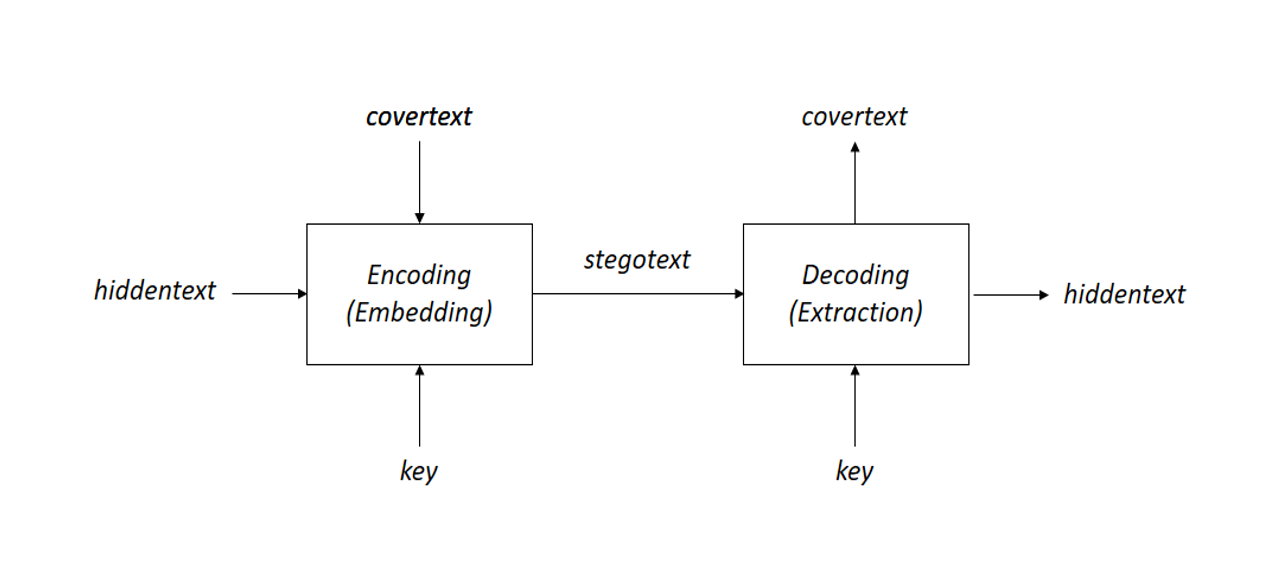
\includegraphics[width=1\textwidth]{gambar/diagram_steganografi}
		\caption{Diagram penyisipan dan ekstraksi pada pesan}
		\label{diagram_steganografi}
	\end{figure} 
	
	Istilah di dalam steganografi:
	\begin{enumerate}
		\item \emph{Covertext} merupakan media atau tempat pesan yang digunakan untuk menyembunyikan \emph{hiddentext}. \emph{Covertext} bisa berupa teks, gambar, audio, video, dll.
		\item \emph{Hiddentext}	atau biasa disebut \emph{embedded message} merupakan pesan atau informasi yang ingin disembunyikan. Contohnya bisa berupa teks, gambar, audio, video, dll.
		\item \emph{Stegotext} merupakan pesan yang sudah berisi \emph{embedded message}.
		\item \emph{Encoding} yaitu penyisipan pesan ke dalam media \emph{covertext}.
		\item \emph{Decoding} yaitu ekstraksi pesan dari \emph{stegotext}.
	\end{enumerate}
	
	Menurut \textbf{Munir}, ada kriteria yang harus diperhatikan dalam penyembunyian pesan, yaitu meliputi \emph{Imperceptible}, \emph{Fidelity}, \emph{Recovery} dan \emph{Capacity}.
	\begin{enumerate}
		\item \emph{Imperceptible}\\ 
		Keberadaan pesan rahasia tidak dapat dipersepsi secara visual atau secara audio. Jika \emph{covertext} berupa \emph{file} citra, maka \emph{stegotext} yang dihasilkan harus sukar dibedakan oleh kasat mata dengan \emph{covertext}-nya. Dan jika \emph{covertext} berupa \emph{file} audio, maka telinga tidak dapat mendeteksi perubahan yang ada pada audio \emph{stegotext}-nya. 
		\item \emph{Fidelity}\\
		Kualitas \emph{file} citra penampung tidak jauh berubah. Setelah penambahan pesan rahasia, citra hasil steganografi masih terlihat dengan baik. Pengamat tidak mengetahui kalau di dalam citra tersebut terdapat pesan rahasia.
		\item \emph{Recovery}\\
		Pesan yang disembunyikan harus dapat diekstrak kembali. Karena tujuan steganografi adalah menyembunyikan pesan atau informasi, maka jika informasi itu dibutuhkan harus dapat diambil kembali untuk dapat digunakan.
		\item \emph{Capacity}\\
		Ukuran pesan yang akan disembunyikan sedapat mungkin besar. Agar dapat memaksimalkan manfaat dari steganografi itu sendiri \cite{munir}.
	\end{enumerate}
	
	\subsection{Sejarah Steganografi}
	Seperti kriptografi, penggunaan steganografi sebetulnya telah digunakan berabad-abad yang lalu bahkan sebelum istilah steganografi itu sendiri muncul. Periode sejarah steganografi dapat dibagi menjadi:
	\begin{enumerate}
		\item Steganografi Kuno (\emph{Ancient Steganography})
			\begin{enumerate}
				\item Steganografi dengan media kepala budak
				
				Ditulis oleh \textbf{Herodatus} (485–525 BC), sejarawan Yunani pada tahun 440 BC di dalam buku: \emph{Histories of Herodatus}). Kisah perang antara kerajaan Persia dan rakyat Yunani. \textbf{Herodatus} menceritakan cara \textbf{Histaiaeus} mengirim pesan kepada \textbf{Aristagoras of Miletus} untuk melawan Persia. 
				
				Caranya adalah dengan dipilih beberapa budak. Kemudian kepala budak tersebut digunduli dan ditulis pesan dengan cara ditato. Setelah pesan dituliskan, budak harus menunggu hingga rambutnya tumbuh kembali. Setelah rambut pada kepala budak tersebut tumbuh, budak dikirim ke tempat penerima. Di sana kepala budak digunduli agar pesan dapat dibaca.
					\begin{figure}[H]
						\centering
						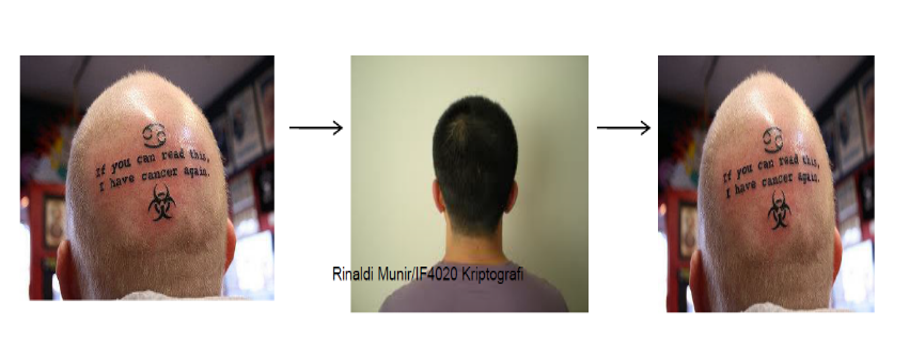
\includegraphics[width=1\textwidth]{gambar/steganografi_kepalabudak}
						\caption{Steganografi dengan media kepala budak}
						\label{steganografi_kepalabudak}
					\end{figure}
				
				\item Penggunaan tablet \emph{wax}
				
				Orang-orang Yunani kuno menulis pesan rahasia di atas kayu yang kemudian ditutup dengan lilin (\emph{wax}). Di dalam bukunya, \textbf{Heradatus} menceritakan \textbf{Demaratus} mengirim peringatan tentang serangan yang akan datang ke Yunani dengan menulis langsung pada tablet kayu yang kemudian dilapisi lilin dari lebah.
					\begin{figure}[H]
						\centering
						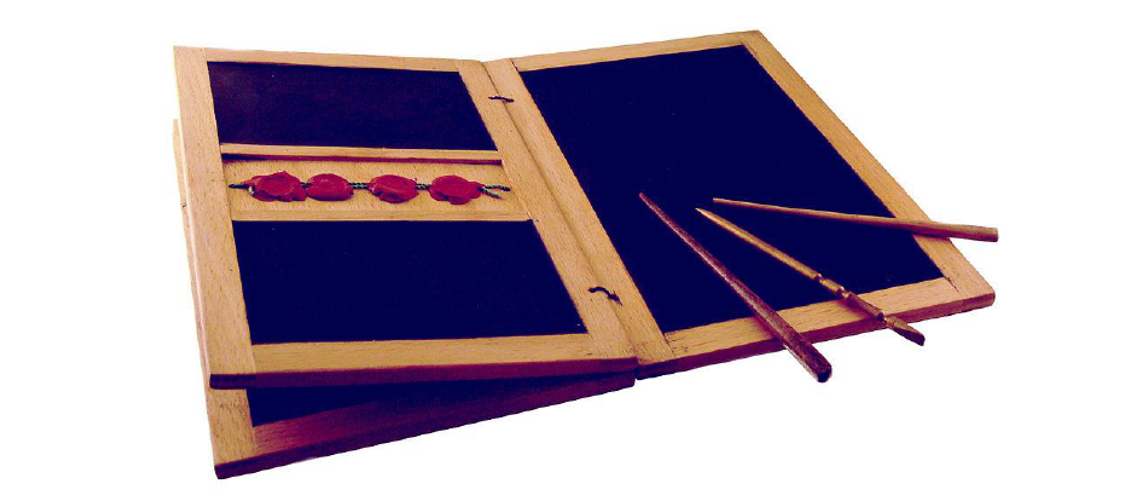
\includegraphics[width=1\textwidth]{gambar/tablet_wax}
						\caption{Tablet \emph{wax}}
						\label{tablet_wax}
					\end{figure}
					
				\item Penggunaan tinta tak-tampak (\emph{invisible ink})
				
				\textbf{Pliny the Elder} menjelaskan penggunaan tinta dari getah tanaman \emph{thithymallus}. Jika dituliskan pada kertas maka tulisan dengan tinta tersebut tidak kelihatan, tetapi bila kertas dipanaskan berubah menjadi gelap/coklat.
				
				\item Penggunaan kain sutra dan lilin
				
				Orang Cina kuno menulis catatan pada potongan-potongan kecil sutra yang kemudian digumpalkan menjadi bola kecil dan dilapisi lilin. Selanjutnya bola kecil tersebut ditelan oleh si pembawa pesan. Pesan dibaca setelah bola kecil dikeluarkan dari perut si pembawa pesan.			
			\end{enumerate}
		\item Steganografi Zaman Renaisans (\emph{Renaissance Steganography})
		
		Tahun 1499, \textbf{Johannes Trithemius} menulis buku \emph{Steganographia}, yang menceritakan tentang metode steganografi berbasis karakter. Selanjutnya tahun 1518 dia menulis buku tentang steganografi dan kriptografi berjudul \emph{Polygraphiae}. \textbf{Giovanni Battista Porta} menggambarkan cara menyembunyikan pesan di dalam telur rebus. Caranya, pesan ditulis pada kulit telur yang dibuat dari tinta khusus yang dibuat dengan satu ons tawas dan setengah liter cuka. Prinsipnya penyembunyiannya adalah tinta tersebut akan menembus kulit telur yang berpori, tanpa meninggalkan jejak yang terlihat. Tulisan dari tinta akan membekas pada permukaan isi telur yang telah mengeras (karena sudah direbus sebelumnya). Pesan dibaca dengan membuang kulit telur.
		
		\item Steganografi Zaman Perang Dunia (\emph{World War Steganography})
		
		\begin{figure}[H]
			\centering
			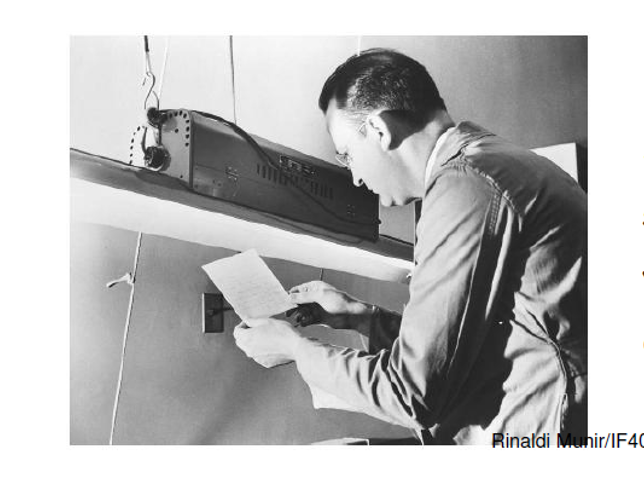
\includegraphics[width=1\textwidth]{gambar/steganografi_perangdunia}
			\caption{Steganografi zaman perang dunia}
			\label{steganografi_perangdunia}
		\end{figure}
	
		Selama terjadinya Perang Dunia ke-2, tinta yang tidak tampak (\emph{invisible ink}) telah digunakan untuk menulis informasi pada lembaran kertas sehingga saat kertas tersebut jatuh di tangan pihak lain hanya akan tampak seperti lembaran kertas kosong biasa. Cairan seperti air kencing (\emph{urine}), susu, vinegar, dan jus buah digunakan sebagai media penulisan sebab bila salah satu elemen tersebut dipanaskan, tulisan akan menggelap dan tampak melalui mata manusia \cite{munir}.
		
		\item Steganografi \emph{Digital}
		
		Sejalan dengan perkembangan maka konsep awal steganografi diimplementasikan pula dalam dunia komputer, yang kemudian dikenal dengan istilah steganografi \emph{digital}. Dalam hal ini, steganografi \emph{digital} memiliki dua properti dasar yaitu media penampung (\emph{cover data} atau \emph{data carrier}) dan data \emph{digital} yang akan disisipkan (\emph{secret data}), dimana media penampung dan data \emph{digital} yang akan disisipkan dapat berupa \emph{file} multimedia (teks/dokumen, citra, audio maupun video). Terdapat dua tahapan umum dalam steganografi \emph{digital}, yaitu proses \emph{embedding} atau \emph{encoding} (penyisipan) dan proses \emph{extracting} atau \emph{decoding} (pemekaran atau pengungkapan kembali (\emph{reveal})). Hasil yang didapat setelah proses \emph{embedding} atau \emph{encoding} disebut \emph{stego object} (apabila media penampung hanya berupa data citra maka disebut \emph{stego image}) \cite{prayudi}.
	\end{enumerate}

	\subsection{Metode Steganografi}
	Berdasarkan ranah operasinya, metode-metode steganografi dapat dibagi menjadi dua kelompok:
	\begin{enumerate}
		\item \emph{Spatial (time) domain methods}\\
		Memodifikasi langsung nilai byte dari \emph{cover-object} (nilai \emph{byte} dapat merepresentasikan intensitas/warna \emph{pixel} atau amplitudo). Contoh: Metode modifikasi LSB
		
		\item \emph{Tranform domain methods}\\
		Memodifikasi hasil transformasi sinyal dalam ranah transform (hasil trnasformasi dari ranah spasial ke ranah lain (misalnya ranah frekuensi). Contoh: Metode \emph{Spread Spectrum} \cite{munir}.
		
	\end{enumerate}

	Ada empat jenis metode steganografi:
	\begin{enumerate}
		\item \emph{Least Significant Bit Insertion} (LSB)\\
		Metode yang digunakan untuk menyembunyikan pesan pada media \emph{digital} tersebut berbeda-beda. Contohnya, pada berkas \emph{image} pesan dapat disembunyikan dengan menggunakan cara menyisipkannya pada bit rendah atau bit yang paling kanan (LSB) pada data \emph{pixel} yang menyusun \emph{file} tersebut. Pada berkas \emph{bitmap} 24 bit, setiap \emph{pixel} (titik) pada gambar tersebut terdiri dari susunan tiga warna \emph{Red}, \emph{Green} dan \emph{Blue} (RGB) yang masing-masing disusun oleh bilangan 8 bit (\emph{byte}) dari 0 sampai 255 atau dengan format biner 00000000 sampai 11111111. Dengan demikian, pada setiap \emph{pixel} berkas \emph{bitmap} 24 bit kita dapat menyisipkan 3 bit data. 
		\item \emph{Algorithms and Transformation}\\
		\emph{Algoritma compression} adalah metode steganografi dengan menyembunyikan data dalam fungsi matematika. Dua fungsi tersebut adalah \emph{Discrete Cosine Transformation} (DCT) dan \emph{Wavelet Transformation}. Fungsi DCT dan \emph{Wavelet} yaitu mentransformasi data dari satu tempat (\emph{domain}) ke tempat (\emph{domain}) yang lain. Fungsi DCT yaitu mentransformasi data dari tempat \emph{spatial} (\emph{spatial domain}) ke tempat frekuensi (\emph{frequency domain}).
		\item \emph{Redundant Pattern Encoding}\\
		\emph{Redundant Pattern Encoding} adalah menggambar pesan kecil pada kebanyakan gambar. Keuntungan dari metode ini adalah dapat bertahan dari \emph{cropping} (kegagalan). Kerugiannya yaitu tidak dapat menggambar pesan yang lebih besar.
		\item \emph{Spread Spectrum Method}\\
		\emph{Spread Spectrum} steganografi terpencar-pencar sebagai pesan yang diacak (\emph{encrypted}) melalui gambar (tidak seperti dalam LSB). Untuk membaca suatu pesan, penerima memerlukan algoritma yaitu \emph{crypto-key} dan \emph{stego-key}. Metode ini juga masih mudah diserang yaitu penghancuran atau pengrusakan dari kompresi dan proses \emph{image} (gambar) \cite{wikipedia1}.
	\end{enumerate}

	Metode LSB dan \emph{Spread Spectrum} adalah dua metode yang sering digunakan dalam melakukan steganografi. Selain karena metodenya yang sederhana, proses \emph{embedding} dan ekstraksi dari kedua metode tersebut juga \emph{relative} cepat\cite{pavani}. Tetapi LSB memiliki proses \emph{embedding} dan ekstraksi yang lebih cepat dari metode \emph{Spread Spectrum} karena proses metode \emph{Spread Spectrum} harus melalui peng-XOR-an antara pesan dan kata kunci, sedangkan LSB langsung menyisipkan pesan ke dalam gambar \cite{pakereng}.
	

\section{Perbedaan Steganografi dan Kriptografi}
Steganografi dan kriptografi mempunyai prinsip kerja yang berbeda, meskipun keduanya mempunyai hubungan yang dekat dalam dunia keamanan data. Pada kriptografi menghasilkan sebuah \emph{chipertext} dimana dengan itu seolah-olah dengan sengaja menunjukkan kepada orang lain bahwa ada sesuatu di dalamnya, namun tidak dapat diketahui maknanya. Namun dengan bentuk \emph{chiper}-nya, justru akan membuat data tersebut terancam oleh usaha-usaha yang dilakukan oleh orang lain untuk dapat membongkarnya dengan tujuan dan atau alasan apapun.
\begin{figure}[H]
	\centering
	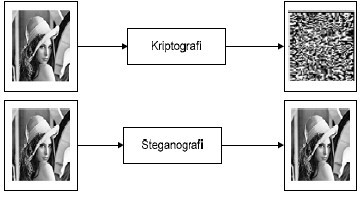
\includegraphics[width=1\textwidth]{gambar/perbedaan_kripsteg}
	\caption{Perbedaan Kriptografi dan Steganografi}
	\label{perbedaan_kripsteg}
\end{figure}

Steganografi dan kriptografi merupakan seni dan teknik yang dapat digunakan untuk melakukan pengamanan data digital. Namun keduanya tidaklah sama. Pada kriptografi, suatu data digital diamankan dengan cara mengenkripsi data tersebut dan menghasilkan sebuah data yang berupa sandi, secara visual data tersebut masih dapat terlihat atau diketahui, hanya saja data tersebut menjadi tidak dapat dimengerti. Berbeda dengan steganografi yang tujuannya adalah menyembunyikan data ke dalam sebuah media yang lain, sehingga data tersebut tidak terlihat \cite{setiana}.

\section{LSB (\emph{Least Significant Bit})}
Penyembunyian data dilakukan dengan mengganti bit-bit data di dalam segmen citra dengan bit-bit rahasia. Pada susunan bit di dalam sebuah \emph{byte} (1 \emph{byte}= 8 bit), ada bit yang paling berarti (\emph{most significant bit} atau MSB) dan bit yang paling kurang berarti (\emph{least significant bit} atau LSB). LSB merupakan salah satu metode yang paling sederhanaa dalam steganografi. Bit yang cocok untuk diganti adalah bit LSB, sebab perubahan tersebut hanya mengubah nilai \emph{byte} satu lebih tinggi atau satu lebih rendah dari nilai sebelumnya \cite{munir}.

Pada \emph{file bitmap} 24 bit, setiap bit masing-masing memiliki komponen \emph{Red, Green,} dan \emph{Blue} (RGB), sehingga dapat menyimpan 3 bit pada setiap \emph{pixel}-nya. Pada gambar 800x600 \emph{pixel} dapat digunakan untuk menyembunyikan 1.440.000 bit (180.000 \emph{Byte}) data rahasia. Sebagai contoh diambil 3 \emph{pixel} dari \emph{file bitmap} 24 bit yang akan disisipkan pesan atau data rahasia karakter "A":
\begin{figure}[H]
	\centering
	(00001000 00101011 11011100)\\
	(11100000 11000100 00010101)\\
	(00010011 10101010 01100011)\\
\end{figure}

Karakter "A" mempunyai nilai biner 01000001, maka bit hasil penyisipannya adalah:
\begin{figure}[H]
	\centering
	(00001000 00101011 11011100)\\
	(11100000 11000100 0001010\textbf{0})\\
	(0001001\textbf{0} 1010101\textbf{1} 01100011\\
\end{figure}

Bit-bit yang nilainya berganti ada 3 dalam 8 \emph{Byte} yang digunakan. Contoh lainnya adalah diambil 8 pixel dari sebuah gambar, maka data rahasia yang dapat dimasukkan adalah 1 kata, contohnya adalah "ADA"
\begin{figure}[H]
	\centering
	(10011011 01100100 01010000)\\
	(10010011 01010101 01001000)\\
	(10011010 01010111 01001110)\\
	(10011010 01010101 01010000)\\
	(10001000 01000001 00111111)\\
	(01101001 00100010 00110100)\\
	(01101101 00100111 00110010)\\
	(01111001 00110011 00110101)\\
\end{figure}

Kata "ADA" mempunyai biner A = 01000001, D = 01000100, maka bit hasil penyisipannya adalah:
\begin{figure}[H]
	\centering
	(1001101\textbf{0} 0110010\textbf{1} 01010000)\\
	(1001001\textbf{0} 0101010\textbf{0} 01001000)\\
	(10011010 01010111 01001110)\\
	(1001101\textbf{1} 0101010\textbf{0} 01010000)\\
	(10001000 01000001 0011111\textbf{0})\\
	(0110100\textbf{0} 00100010 0011010\textbf{1})\\
	(0110110\textbf{0} 0010011\textbf{0} 00110010)\\
	(0111100\textbf{0} 0011001\textbf{0} 00110101)\\
\end{figure}

Bit-bit yang nilainya berganti ada 13 dalam 24 \emph{Byte} yang digunakan. Secara rata-rata, LSB hanya menggunakan setengah dari bit dalam gambar yang perlu dimodifikasi untuk menyembunyikan pesan rahasia. Perubahan ini tidak dapat dirasakan oleh mata manusia, dan pesan berhasil disembunyikan \cite{elgabar2}.

\section{ASCII}
ASCII adalah singkatan dari \emph{American Standard Code for Information Interchange}. Komputer hanya dapat memahami angka, jadi kode ASCII adalah representasi numerik dari karakter seperti 'a' atau '@' atau karakter lainnya. Kode ASCII memiliki komposisi bilangan biner sebanyak 8 bit. Dimulai dari 00000000 hingga 11111111. Total kombinasi yang dihasilkan ASCII sebanyak 256, dimulai dari kode 0 hingga 255 dalam sistem bilangan desimal. \cite{ascii}
\begin{table}[H]
	\centering
	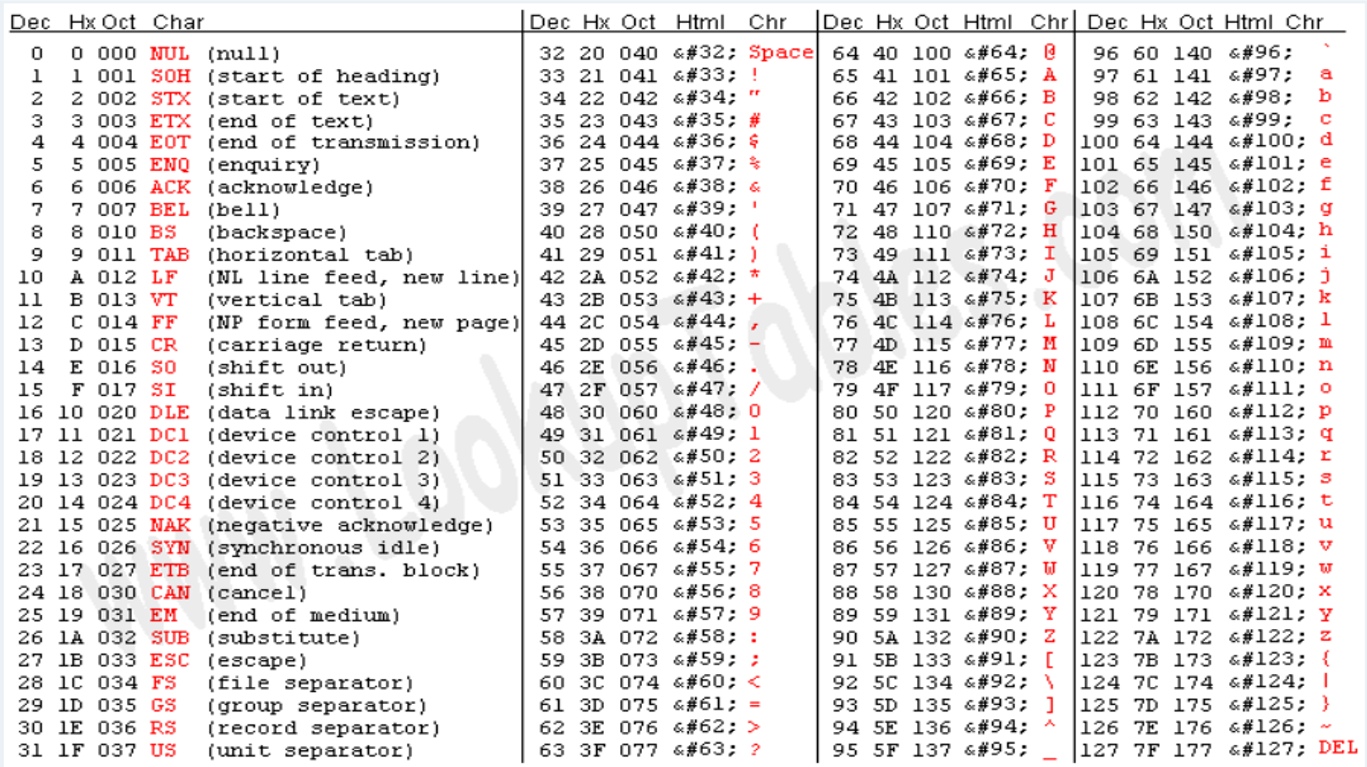
\includegraphics[width=1.0\textwidth]{gambar/table_ascii}
	\caption{Tabel ASCII}
	\label{tabel_ascii}
\end{table}

\section{\emph{Citra Digital}}
	\subsection{Pengertian Citra \emph{Digital}}
	Citra atau gambar dapat didefinisikan sebagai sebuah fungsi dua dimensi, f(x,y), x dan y adalah koordinat bidang datar; dan harga fungsi f di setiap pasangan koordinat (x,y) disebut intensitas atau level keabuan (\emph{grey level}) dari gambar di titik itu \cite{hermawati}. Citra \emph{digital} merupakan suatu \emph{array} dua dimensi atau suatu matriks yang elemen-elemennya menyatakan tingkat keabuan dari elemen gambar \cite{arymurthy} 
	
	Ada 3 bidang studi utama yang menangani pengolahan data atau informasi berbentuk gambar atau citra, yaitu:
	\begin{enumerate}
		\item Grafika Komputer (\emph{Computer Graphics})
		\item Pengolahan Citra (\emph{Image Processing})
		\item Pengenalan Pola (\emph{Pattern Recognition})
	\end{enumerate}
	
	\subsection{Pengolahan Citra (\emph{Image Processing})}
	Pengolahan citra adalah pemrosesan citra, khususnya dengan menggunakan komputer, menjadi citra yang kualitasnya lebih baik. Pengolahan Citra bertujuan memperbaiki kualitas citra agar mudah diinterpretasi oleh manusia atau mesin (dalam hal ini komputer). Teknik-teknik pengolahan citra mentransformasikan citra menjadi citra lain. Jadi, masukannya adalah citra dan keluarannya juga citra, namun citra keluaran mempunyai kualitas lebih baik daripada citra masukan \cite{munir04}
	
	\subsection{Format \emph{File} pada Citra \emph{Digital}}
		\begin{enumerate}
			\item BMP\\
			BMP adalah singkatan dari \emph{Bitmap} yang dahulu dikembangkan oleh MICROSOFT. \emph{Bitmap} dapat menyimpan data warna untuk masing-masing \emph{pixel} dalam gambar tanpa kompresi apapun. Format ini dapat digunakan untuk menyembunyikan data tanpa menaikkan kecurigaan pada mata manusia. Gambar yang dihasilkan tanpa kompresi dan format \emph{lossless} yang merupakan salah satu faktor penting. Ekstensi yang digunakan dalam \emph{file} ini adalah .bmp \cite{gautam}.
			\item JPEG\\
			Istilah JPEG sebenarnya adalah singkatan dari pengembangnya, yaitu \emph{Joint Photographic Experts Group}. Gambar JPEG tidak terbatas pada sejumlah warna tertentu. Oleh karena itu, format JPEG paling baik untuk mengompresi gambar foto. Gambar dengan format JPEG dapat berisi data gambar beresolusi tinggi berwarna-warni, itu adalah format \emph{lossy}, yang berarti beberapa kualitas hilang ketika gambar dikompresi. Jika gambar terlalu banyak dikompres, grafiknya menjadi seperti "tidak berwarna" dan sebagian detailnya hilang. Ekstensi yang digunakan dalam \emph{file} ini adalah .jpeg \cite{elgabar}.
			\item GIF\\
			GIF adalah singkatan dari \emph{Graphics Interchange Format} yang dikembangkan oleh COMPUSERVICE. GIF digunakan untuk tujuan menyimpan beberapa gambar \emph{bitmap} dalam satu \emph{file} gambar. GIF sering digunakan untuk menyimpan grafik multi-bit dan data gambar. GIF tidak terkait dengan aplikasi perangkat lunak tertentu tetapi dirancang untuk memudahkan pertukaran dan tampilan data gambar yang tersimpan di lokal atau sistem komputer jarak jauh. GIF digunakan juga karena menerapkan metode kompresi \emph{lossless}. Ekstensi yang digunakan dalam \emph{file} ini adalah .gif \cite{elgabar2}.
			\item TIFF\\
			TIFF adalah singkatan dari \emph{Taged Image Format File}. TIFF dikembangkan oleh ADOBE dan digunakan untuk grafis berkualitas tinggi dengan kompresi \emph{lossless}. Format \emph{file} ini memiliki transparansi dan pilihan warna terindeks untuk menanamkan pesan rahasia di atasnya. TIFF mendukung properti RGB dan \emph{GRAYSCALE} dan digunakan untuk HD \emph{Imaging}. Ini adalah salah satu format \emph{file} paling serbaguna di antara semua format yang tersedia. Ekstensi yang digunakan dalam format \emph{file} ini adalah .tiff \cite{gautam}.
			\item PNG\\
			PNG adalah singkatan dari \emph{Portable Network Graphics} yang dikembangkan oleh PNG \emph{Development Group}. PNG mampu menyembunyikan pesan yang besar di dalamnya. Format \emph{file} ini diciptakan untuk meningkatkan format \emph{file} gambar GIF menghilangkan batasan 256 warna tetapi tidak mendukung animasi. Dan PNG menggunakan kompresi data \emph{lossless}. Ekstensi yang digunakan dalam format \emph{file} ini adalah .png \cite{gautam}.
		\end{enumerate}
	Perbedaan komponen antara masing-masing format \emph{file} citra \emph{digital} dapat dilihat pada Tabel \ref{tabel_perbedaan}. 
	\begin{table}[H]
		\centering
		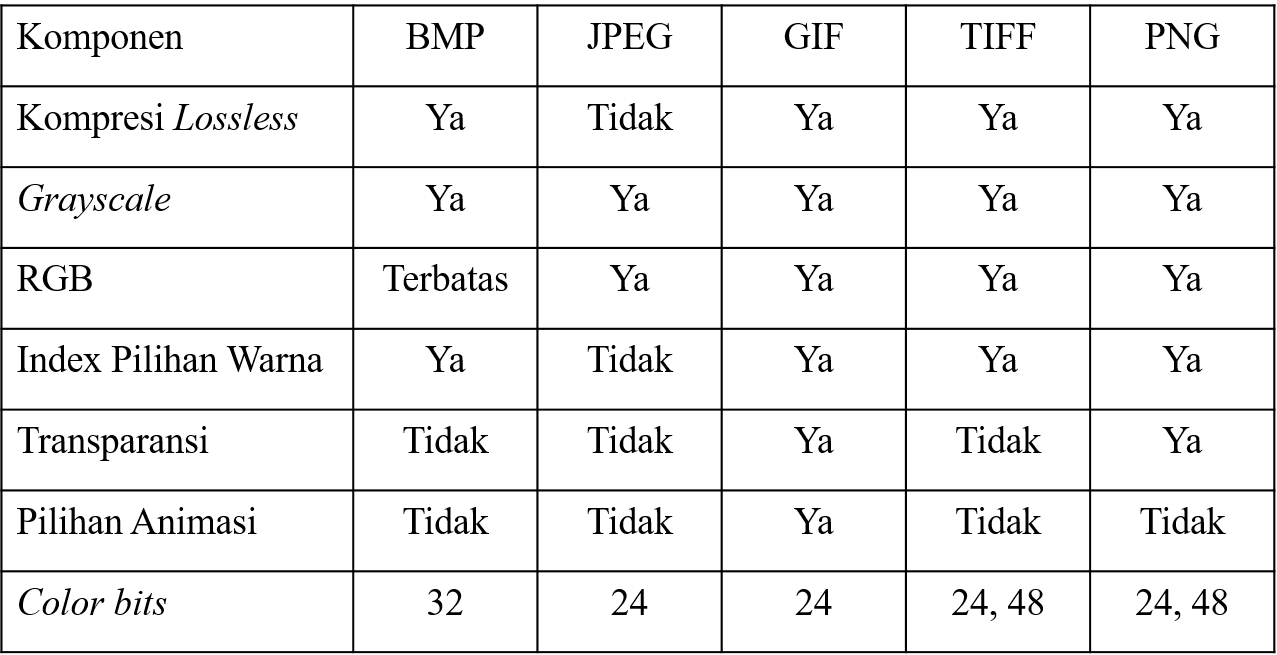
\includegraphics[width=0.8\textwidth]{gambar/table_perbedaan}
		\caption{Perbedaan \emph{file} citra \emph{digital}}
		\label{tabel_perbedaan}
	\end{table}

\section{Konsep RAD}
	\subsection{Tahapan-Tahapan RAD}
	\subsection{Keunggulan RAD}

% Baris ini digunakan untuk membantu dalam melakukan sitasi
% Karena diapit dengan comment, maka baris ini akan diabaikan
% oleh compiler LaTeX.
\begin{comment}
bibliography{daftar-pustaka}
\end{comment}


%!TEX root = ./template-skripsi.tex
%-------------------------------------------------------------------------------
%                            BAB III
%               			PEMBAHASAN
%-------------------------------------------------------------------------------

\chapter{HASIL DAN PEMBAHASAN}

Dalam penelitian ini tahapan yang akan dilakukan adalah seperti Gambar 3.1 di bawah ini

\begin{figure}[H]
	\centering
	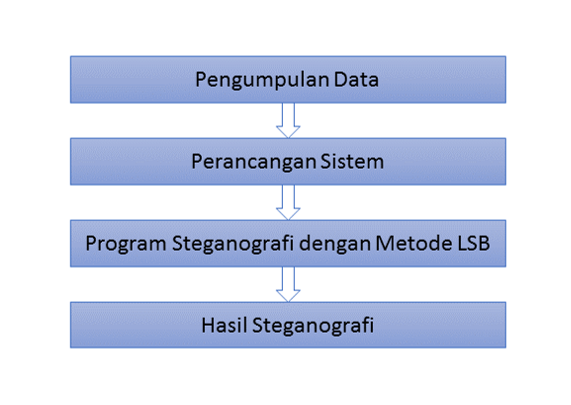
\includegraphics[width=0.8\textwidth]{gambar/alur_penelitian}
	\caption{Alur Penelitian}
	\label{alur_penelitian}
\end{figure}

\section{Pengumpulan Data}
\begin{enumerate}
	\item Studi Pustaka\\
	Penulis mendapatkan informasi yang berkaitan dengan steganografi melalui buku referensi dan juga dalam bentuk \emph{e-book}. Penulis juga mencari informasi melalui berbagai situs di internet yang sesuai dengan topik.	
	\item Studi Literatur\\
	Penulis mencoba mencari perbandingan dengan studi sejenis dari beberapa karya ilmiah lokal maupun internasional, seperti jurnal dan skripsi.	 
\end{enumerate}

\section{Perancangan Sistem}

	\subsection{Proses Penyisipan (\emph{Encoding}) pesan ke Citra \emph{Digital}}
	
	\begin{figure}[H]
		\centering
		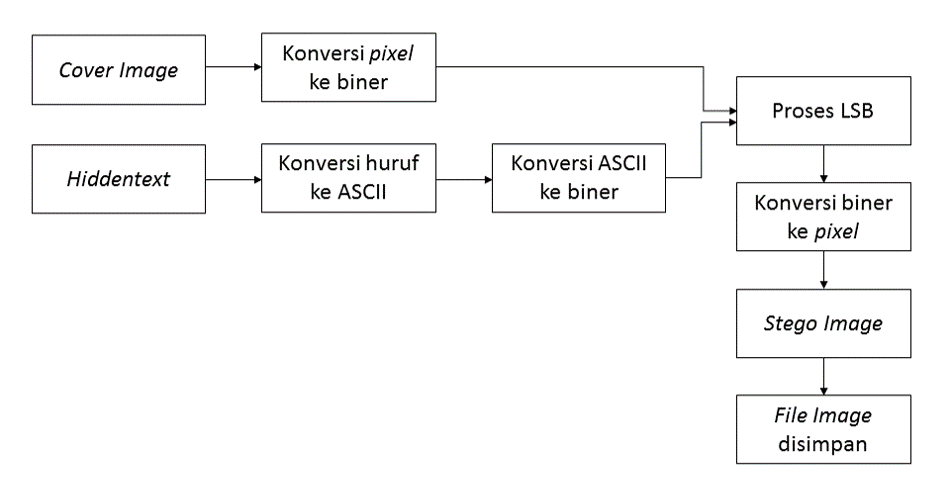
\includegraphics[width=1\textwidth]{gambar/penyisipan2}
		\caption{\emph{Flowchart} Penyisipan Pesan Rahasia}
		\label{flowchart_penyisipan}
	\end{figure}

	Gambar 3.2 adalah \emph{flowchart} proses penyisipan pesan ke dalam \emph{file}
	citra (\emph{Cover Image}). Dimulai dengan membaca \emph{file} citra RGB \emph{Cover Image}. Untuk \emph{file} bitmap RGB maka setiap \emph{pixel} (titik) pada gambar tersebut terdiri dari susunan tiga warna \emph{Red, Green} dan \emph{Blue} yang masing-masing disusun oleh bilangan 8 bit (1 \emph{byte}) dari 0 sampai 255 atau dengan format biner 00000000 sampai 11111111. Setelah membaca \emph{pixel} dari \emph{file} citra langkah selanjutnya menentukan bit terkecil (LSB) pada \emph{Cover Image}.
	
	Secara paralel pesan (\emph{Hiddentext}) dimasukkan. Pesan tersebut dikonversi terlebih dahulu menjadi nilai ASCII dan kemudian dikonversi kembali menjadi nilai Biner. Setelah itu terjadilah proses penyisipan (\emph{Encoding}) antara biner dari \emph{Cover Image} dengan biner dari \emph{Hiddentext}. Selanjutnya biner yang telah disisipkan akan dikonversikan kembali ke dalam \emph{pixel}. Dan menyimpan citra yang telah disisipkan pesan ke dalam \emph{Cover Image} sehingga diperoleh atau	dapat ditampilkan sebuah gambar baru (\emph{Stego Image}).
	
	\subsection{Proses Ekstraksi (\emph{Decoding}) pesan dari Citra \emph{Digital}}
	
	\begin{figure}[H]
		\centering
		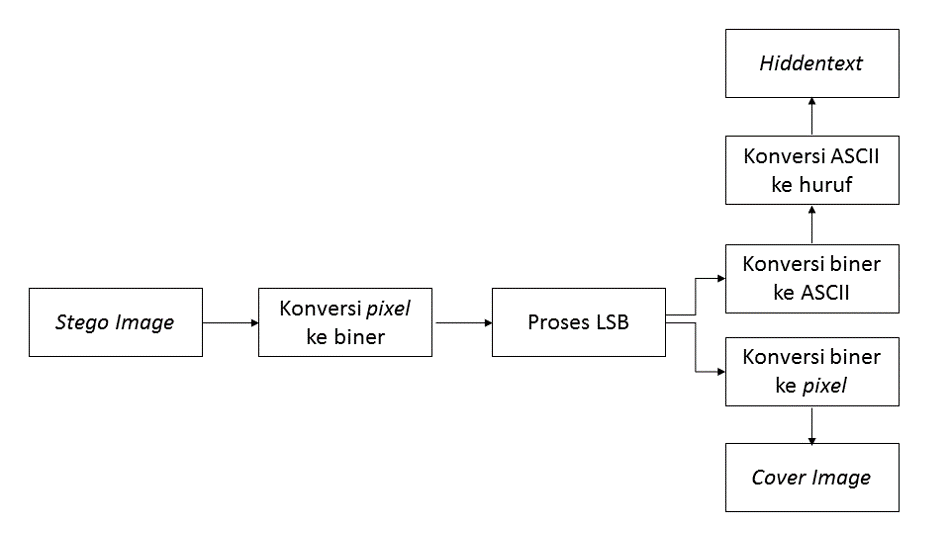
\includegraphics[width=1\textwidth]{gambar/ekstraksi2}
		\caption{\emph{Flowchart} Ekstraksi Pesan Rahasia}
		\label{flowchart_ekstraksi}
	\end{figure}

	Gambar 3.3 adalah \emph{flowchart} proses ekstraksi pesan dari \emph{Stego Image} yang menghasilkan \emph{Hiddentext} yang terdapat di dalamnya. Prosesnya dimulai dengan membaca \emph{file} citra (\emph{Stego Image}), dan mengubah \emph{pixel} ke dalam nilai biner. Kemudian proses ekstraksi (\emph{Decoding}). Setelah diperoleh bit-bit yang tersembunyi pada \emph{Cover Image} maka proses berikutnya adalah mengkonversi kembali pesan yang tersembunyi (\emph{Hiddentext}), sehingga pesan dapat ditampilkan kembali.

	\subsection{Desain Antar Muka Program}
	
	Berikut adalah GUI dari program steganografi yang dibangun dengan menggunakan MATLAB R2016b.
	
	\begin{figure}[H]
		\centering
		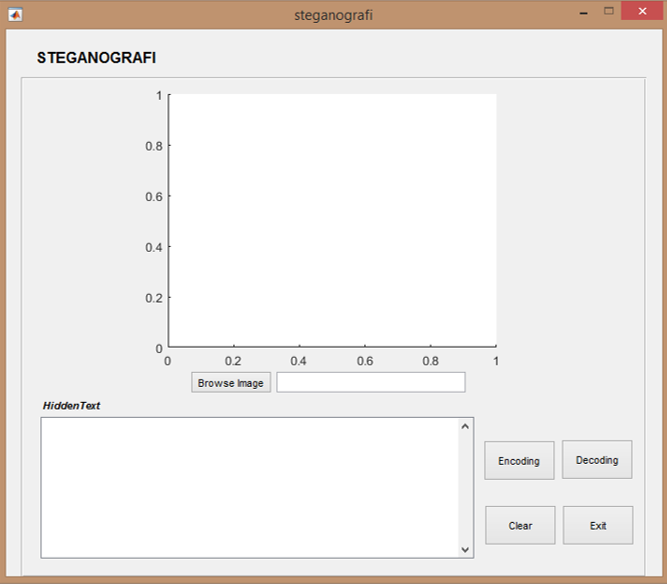
\includegraphics[width=1\textwidth]{gambar/mockup/1}
		\caption{GUI Steganografi}
		\label{desain_form}
	\end{figure}

	Dari Gambar 3.4 tersebut, pengambilan gambar yang akan dijadikan sebagai \emph{Cover Image} dilakukan dengan menekan tombol "\emph{Browse Image}" dan gambar akan tampil. 
	
	\begin{figure}[H]
		\centering
		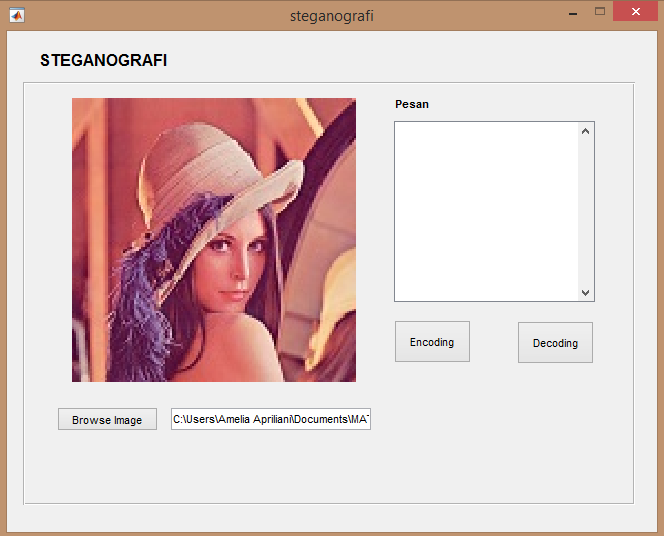
\includegraphics[width=1\textwidth]{gambar/mockup/2}
		\caption{GUI - \emph{Cover Image}}
		\label{desain_image}
	\end{figure}

	Setelah \emph{Cover Image} tampil seperti pada Gambar 3.5 maka pesan yang akan disisipkan atau \emph{Hiddentext} dapat dituliskan pada kolom pesan. Kemudian klik tombol \emph{Encoding} (Gambar 3.6) untuk melakukan proses \emph{Encoding}. Setelah proses \emph{Encoding}, maka akan didapatkan \emph{Stego Image} dan disimpan di dalam folder.
	
	\begin{figure}[H]
		\centering
		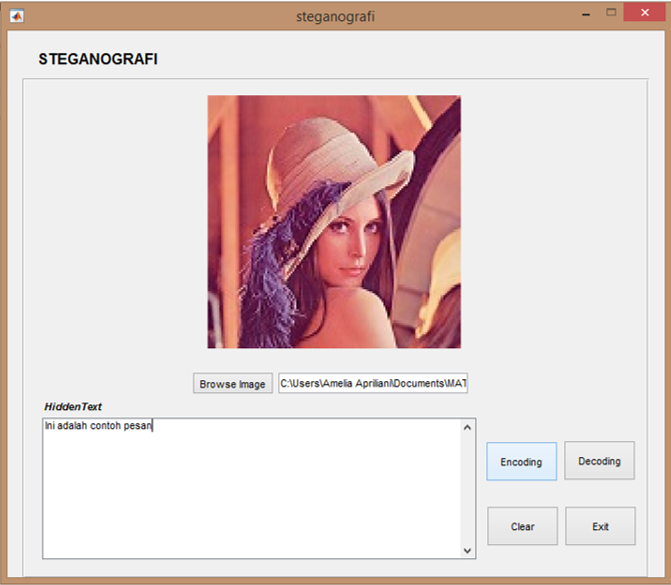
\includegraphics[width=1\textwidth]{gambar/mockup/3}
		\caption{GUI - Proses \emph{Encoding}}
		\label{desain_encoding}
	\end{figure}

	Jika ingin melakukan proses \emph{Decoding}, maka buka \emph{Stego Image} yang telah disimpan. Kemudian klik tombol \emph{Decoding} dan pesan akan didapatkan seperti pada Gambar 3.7.

	\begin{figure}[H]
		\centering
		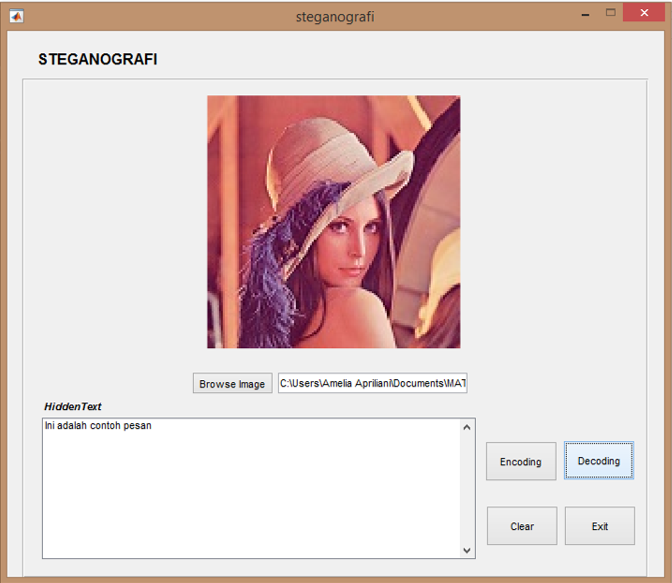
\includegraphics[width=1\textwidth]{gambar/mockup/5}
		\caption{GUI - Pesan Hasil \emph{Decoding}}
		\label{desain_pesan}
	\end{figure}

\section{Program Steganografi dengan Metode LSB}
Program diawali dengan pengambilan \emph{file} citra \emph{digital} yang akan digunakan, berikut adalah \emph{source code}-nya:
	\begin{figure}[H]
		\centering
		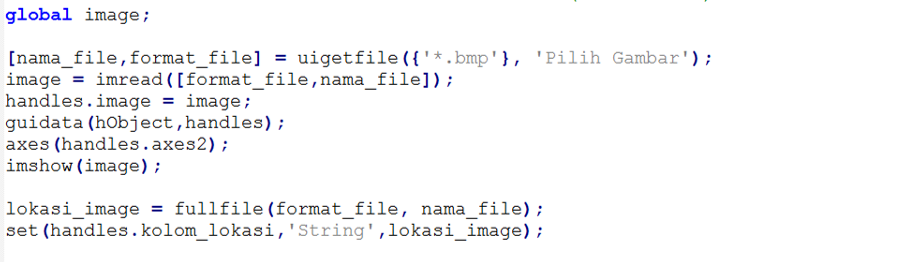
\includegraphics[width=1\textwidth]{gambar/sourcecode/browse_image}
		\caption{\emph{Source Code} - \emph{Browse Image}}
		\label{browse_image}
	\end{figure}

Selanjutnya adalah memasukkan pesan atau \emph{Hiddentext}. \emph{Hiddentext} yang akan dimasukkan tidak boleh melebihi batas maksimal karakter. Panjang karakter maksimal disesuaikan dengan besar \emph{pixel} pada \emph{file} citra. Panjang karakter maksimal dapat dihitung, berikut adalah \emph{source code}-nya:
	\begin{figure}[H]
		\centering
		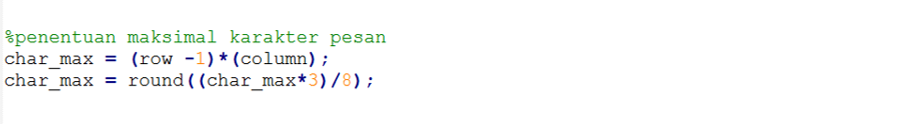
\includegraphics[width=1\textwidth]{gambar/sourcecode/karakter_maksimal}
		\caption{\emph{Source Code} - Menghitung Karakter Maksimal}
		\label{karakter_max}
	\end{figure}

Sedangkan untuk menghitung panjang \emph{hiddentext} yang telah dimasukkan adalah sebagai berikut:
	\begin{figure}[H]
		\centering
		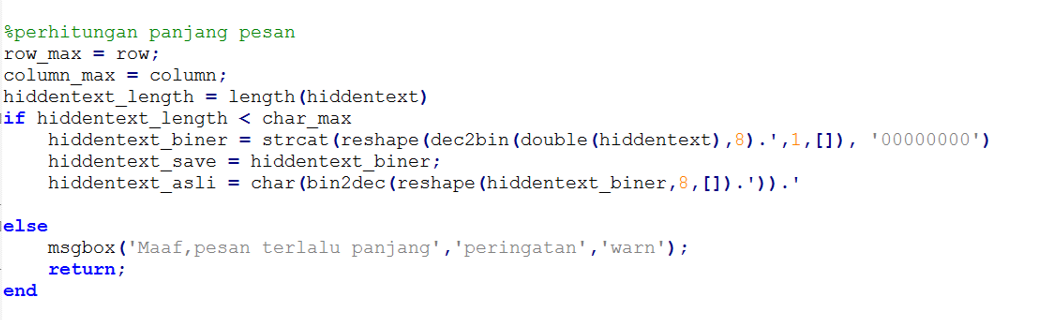
\includegraphics[width=1\textwidth]{gambar/sourcecode/panjang_pesan}
		\caption{\emph{Source Code} - Menghitung Panjang \emph{Hiddentext} yang Dimasukkan}
		\label{panjang_pesan}
	\end{figure}

\subsection{\emph{Encoding}}
Pada tugas akhir ini metode yang digunakan dalam steganografi adalah metode LSB. Proses \emph{Encoding} merupakan proses penyisipan pesan atau \emph{Hiddentext} ke dalam \emph{file} citra. Berikut adalah cuplikan \emph{source code} proses \emph{Encoding} dengan menggunakan metode LSB:
	\begin{figure}[H]
		\centering
		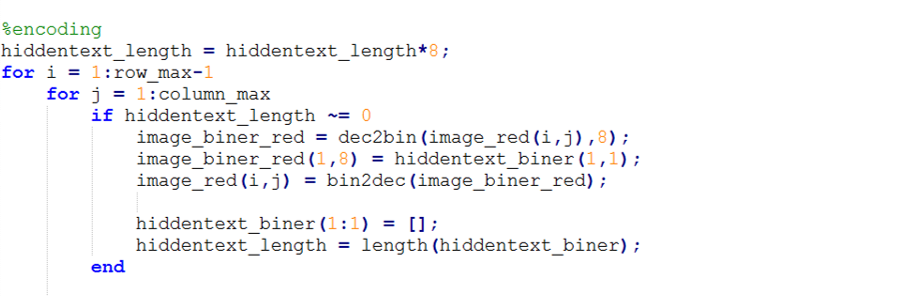
\includegraphics[width=1\textwidth]{gambar/sourcecode/cuplikan_encoding}
		\caption{\emph{Source Code} - Cuplikan \emph{Encoding}}
		\label{cuplikan_encoding}
	\end{figure}

\subsection{\emph{Decoding}}
Proses \emph{Decoding} merupakan proses pengambilan kembali pesan atau \emph{Hiddentext} yang telah disisipkan ke dalam \emph{file} citra. Berikut merupakan cuplikan dari \emph{source code} proses \emph{Decoding}:
	\begin{figure}[H]
		\centering
		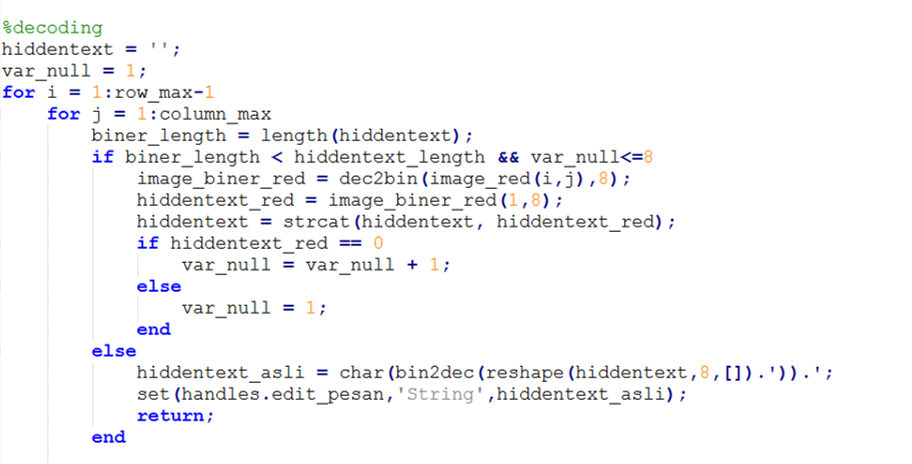
\includegraphics[width=1\textwidth]{gambar/sourcecode/cuplikan_decoding}
		\caption{\emph{Source Code} - Cuplikan \emph{Decoding}}
		\label{cuplikan_decoding}
	\end{figure}
	
\section{Hasil Steganografi}
Setelah dilakukan pengujian terhadap program Steganografi, maka didapatkan hasil sebagai berikut:
	\subsection{Pengujian Berdasarkan Bit pada \emph{File} Citra}
	Pengujian ini menguji berapakah batas Bit \emph{File} Citra yang bisa dimasukkan di dalam program.
	
	%masukkin table
	\begin{table}[H]
		\centering
		\caption{Bit pada \emph{File} Citra}
		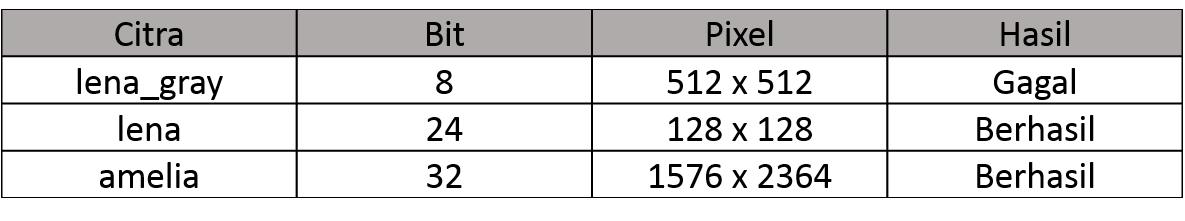
\includegraphics[width=1.0\textwidth]{gambar/table_bitcitra}
		\label{tabel_bitcitra}
	\end{table}
	
	Pada Tabel 3.1 terlihat bahwa \emph{file} citra dengan ukuran 8 bit tidak berhasil untuk disisipkan pesan karena tidak mengandung komponen RGB. Sedangkan untuk \emph{file} citra 24 dan 32 bit bisa digunakan sebagai \emph{Cover Image} untuk menyisipkan pesan karena mengandung komponen RGB didalamnya.
	
	\begin{figure}[H]
		\centering
		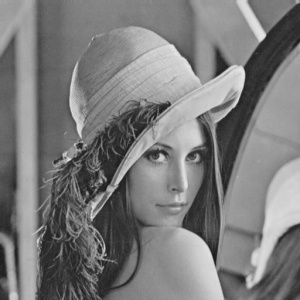
\includegraphics[width=0.4\textwidth]{gambar/matlab/lena_gray}
		\caption{\emph{File} Citra 8 Bit}
		\label{lena_gray8}
	\end{figure}
	
	\begin{figure}[H]
		\centering
		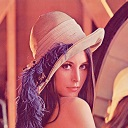
\includegraphics[width=0.4\textwidth]{gambar/matlab/lena}
		\caption{\emph{File} Citra 24 Bit}
		\label{lena24}
	\end{figure}

	\begin{figure}[H]
		\centering
		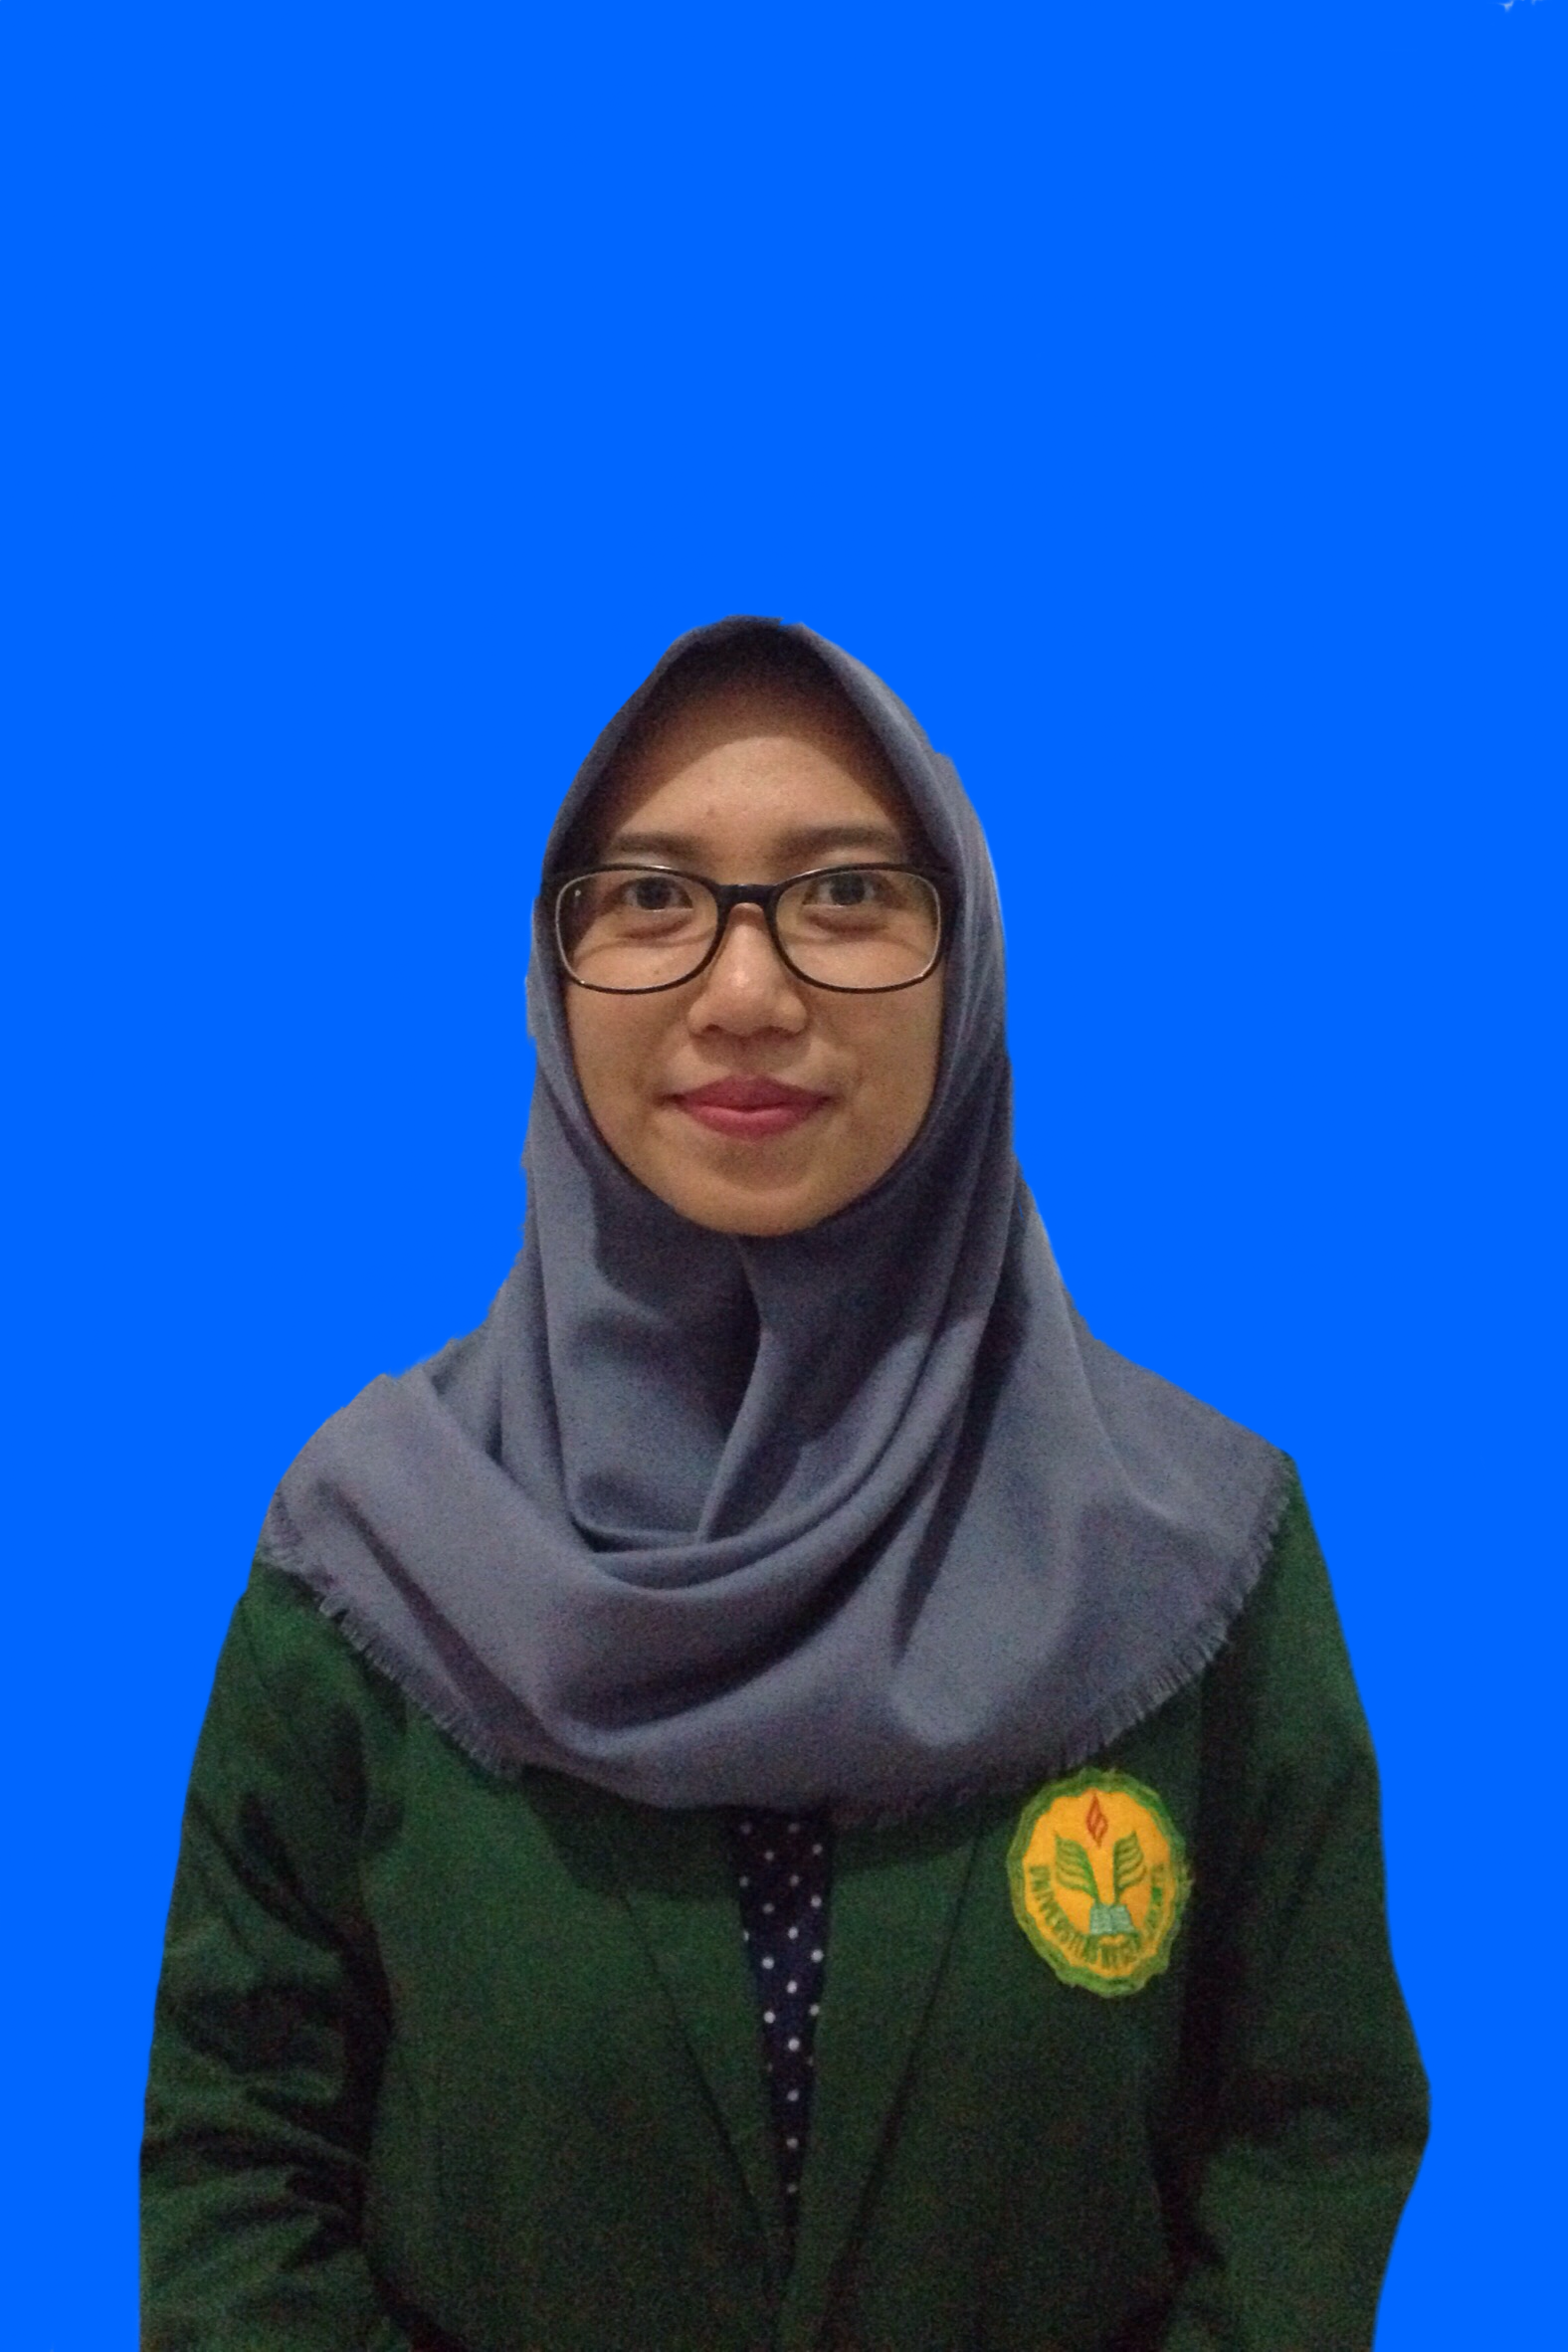
\includegraphics[width=0.4\textwidth]{gambar/matlab/amelia}
		\caption{\emph{File} Citra 32 Bit}
		\label{amelia32}
	\end{figure}

	\subsection{Pengujian Berdasarkan \emph{Imperceptible}}
	Pengujian ini menguji kualitas citra \emph{digital}, apakah citra \emph{digital} akan mengalami perubahan yang mencurigakan atau tidak secara visual. Pengujian ini dikatakan berhasil apabila kualitas dari \emph{Stego Image} yang dihasilkan tidak berbeda jika dibandingkan dengan berkas aslinya atau \emph{Cover Image}.

	%gambar cover
	\begin{figure}[H]
		\centering
		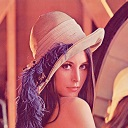
\includegraphics[width=0.4\textwidth]{gambar/matlab/lena}
		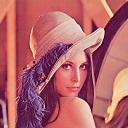
\includegraphics[width=0.4\textwidth]{gambar/matlab/lena_kalimat}
		\caption{Perbandingan \emph{File} Citra - lena.bmp}
		\label{lena_stego}
	\end{figure}

	%gambar cover
	\begin{figure}[H]
		\centering
		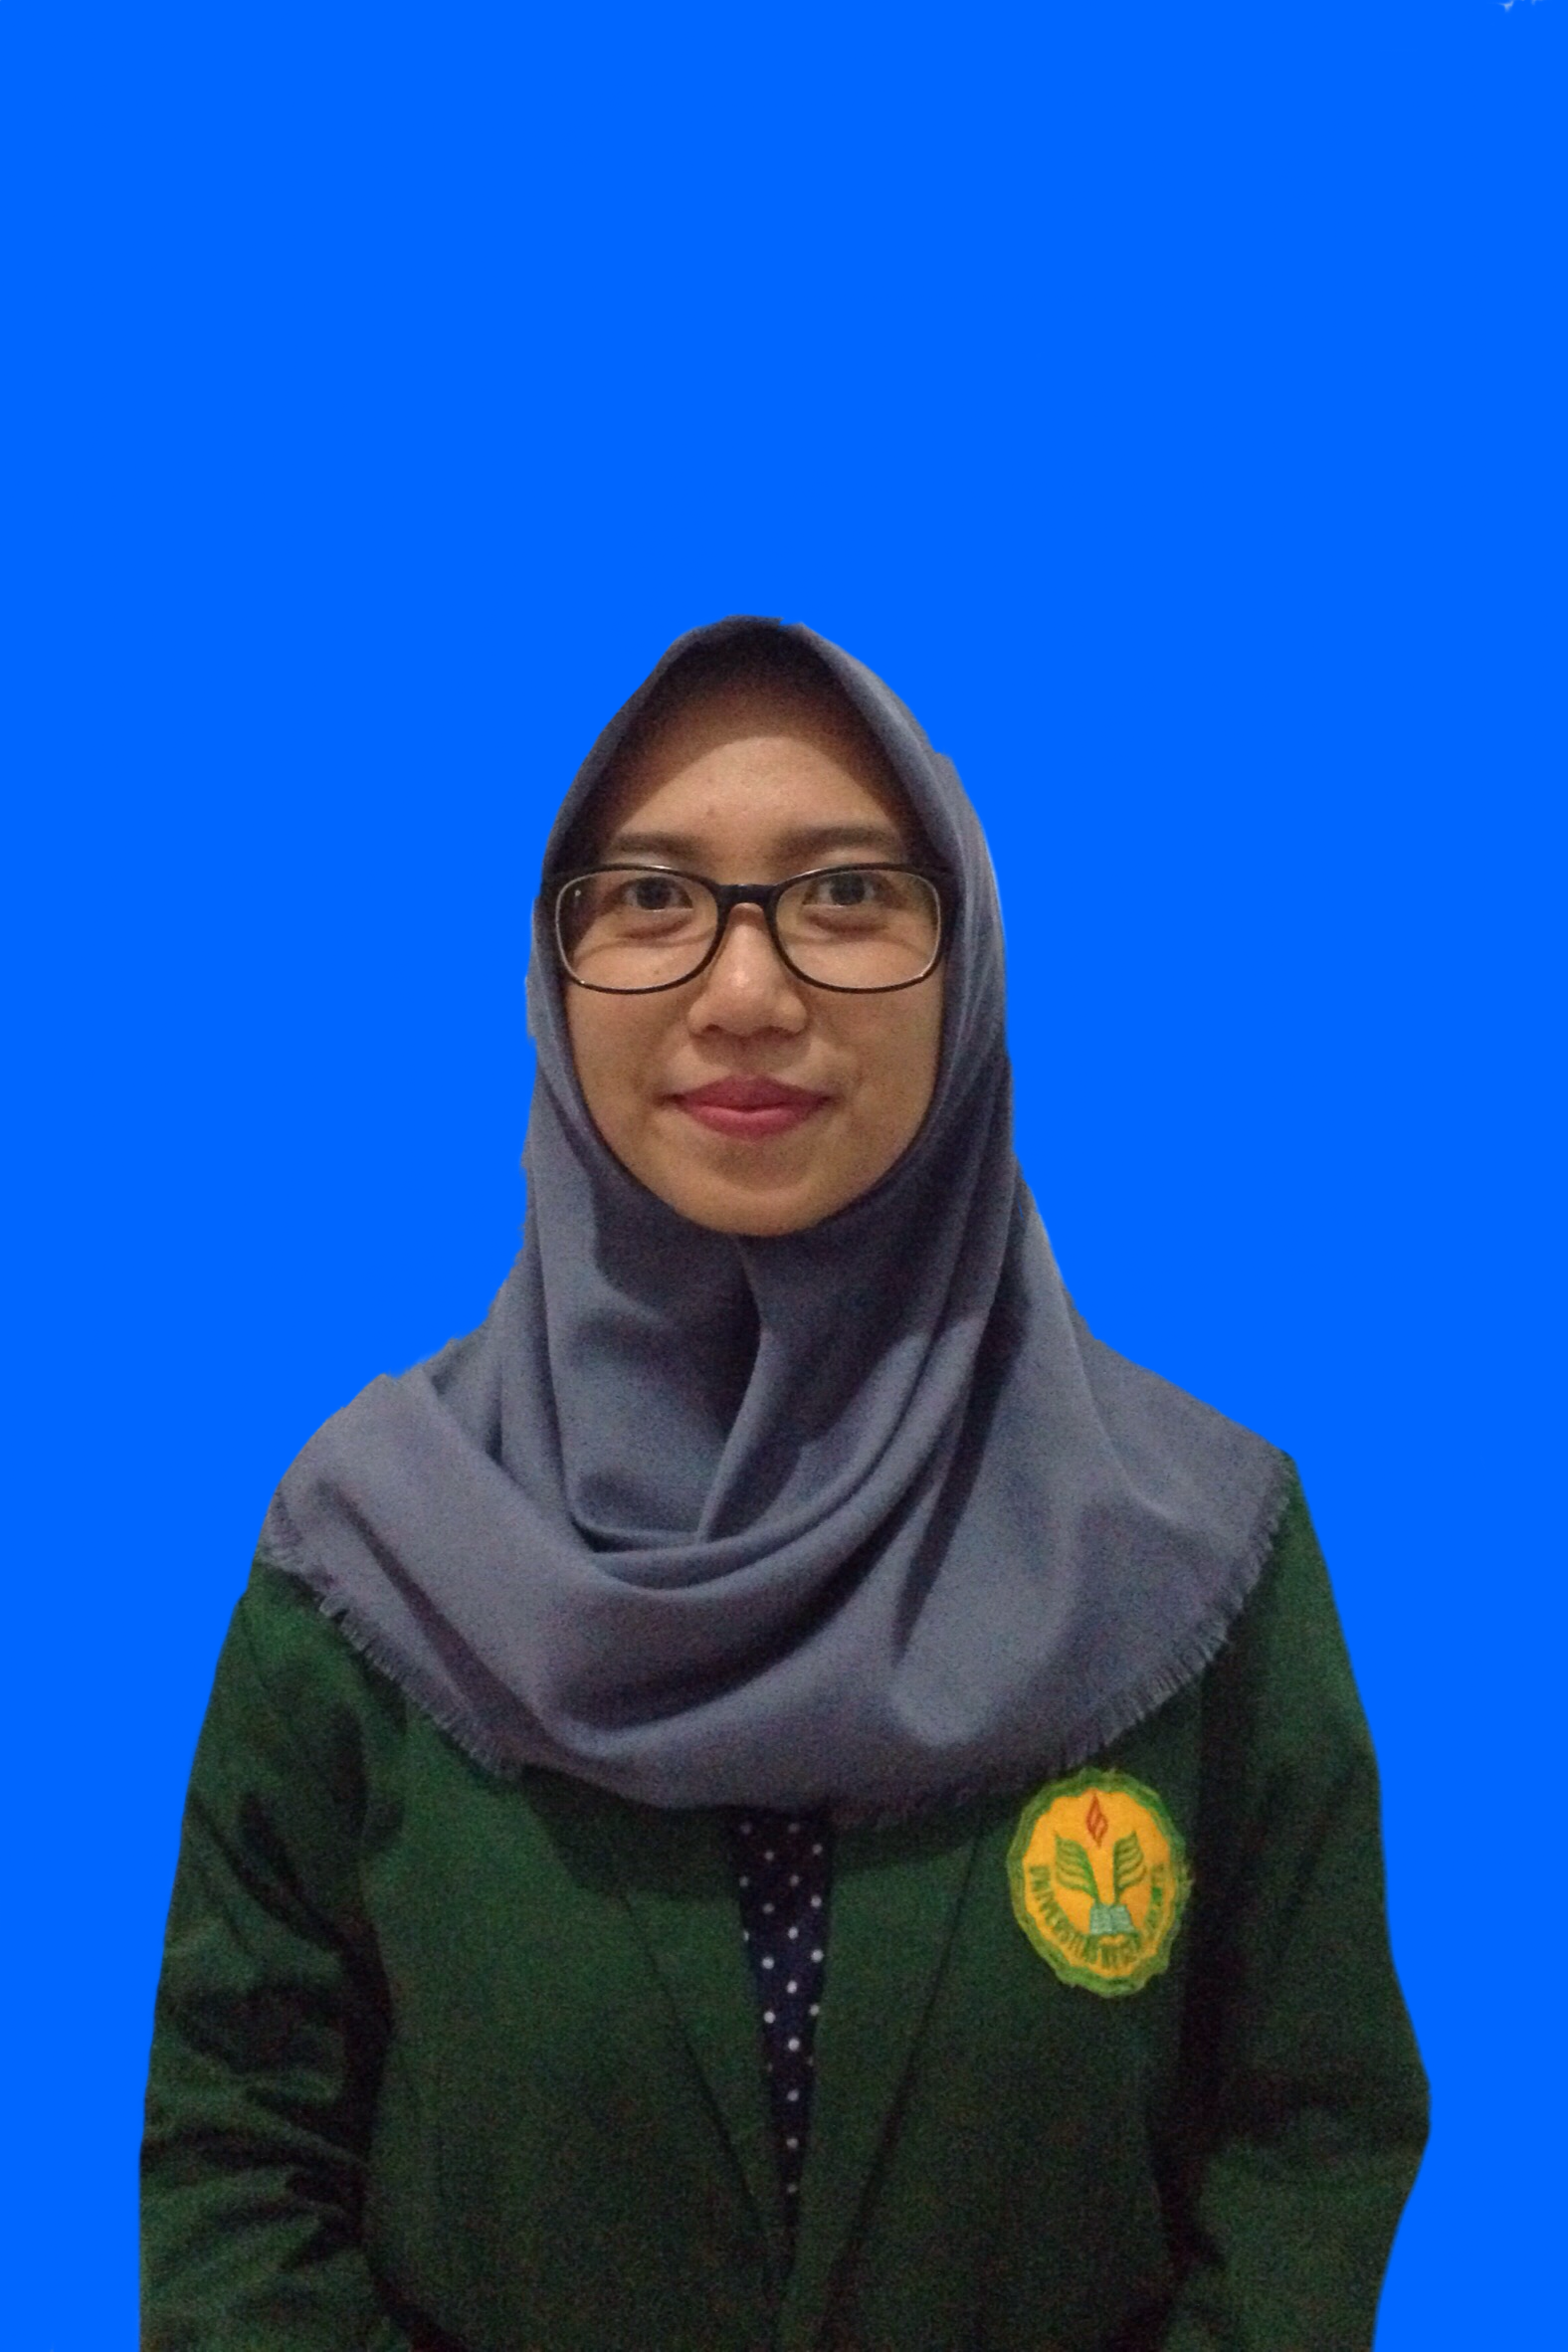
\includegraphics[width=0.4\textwidth]{gambar/matlab/amelia}
		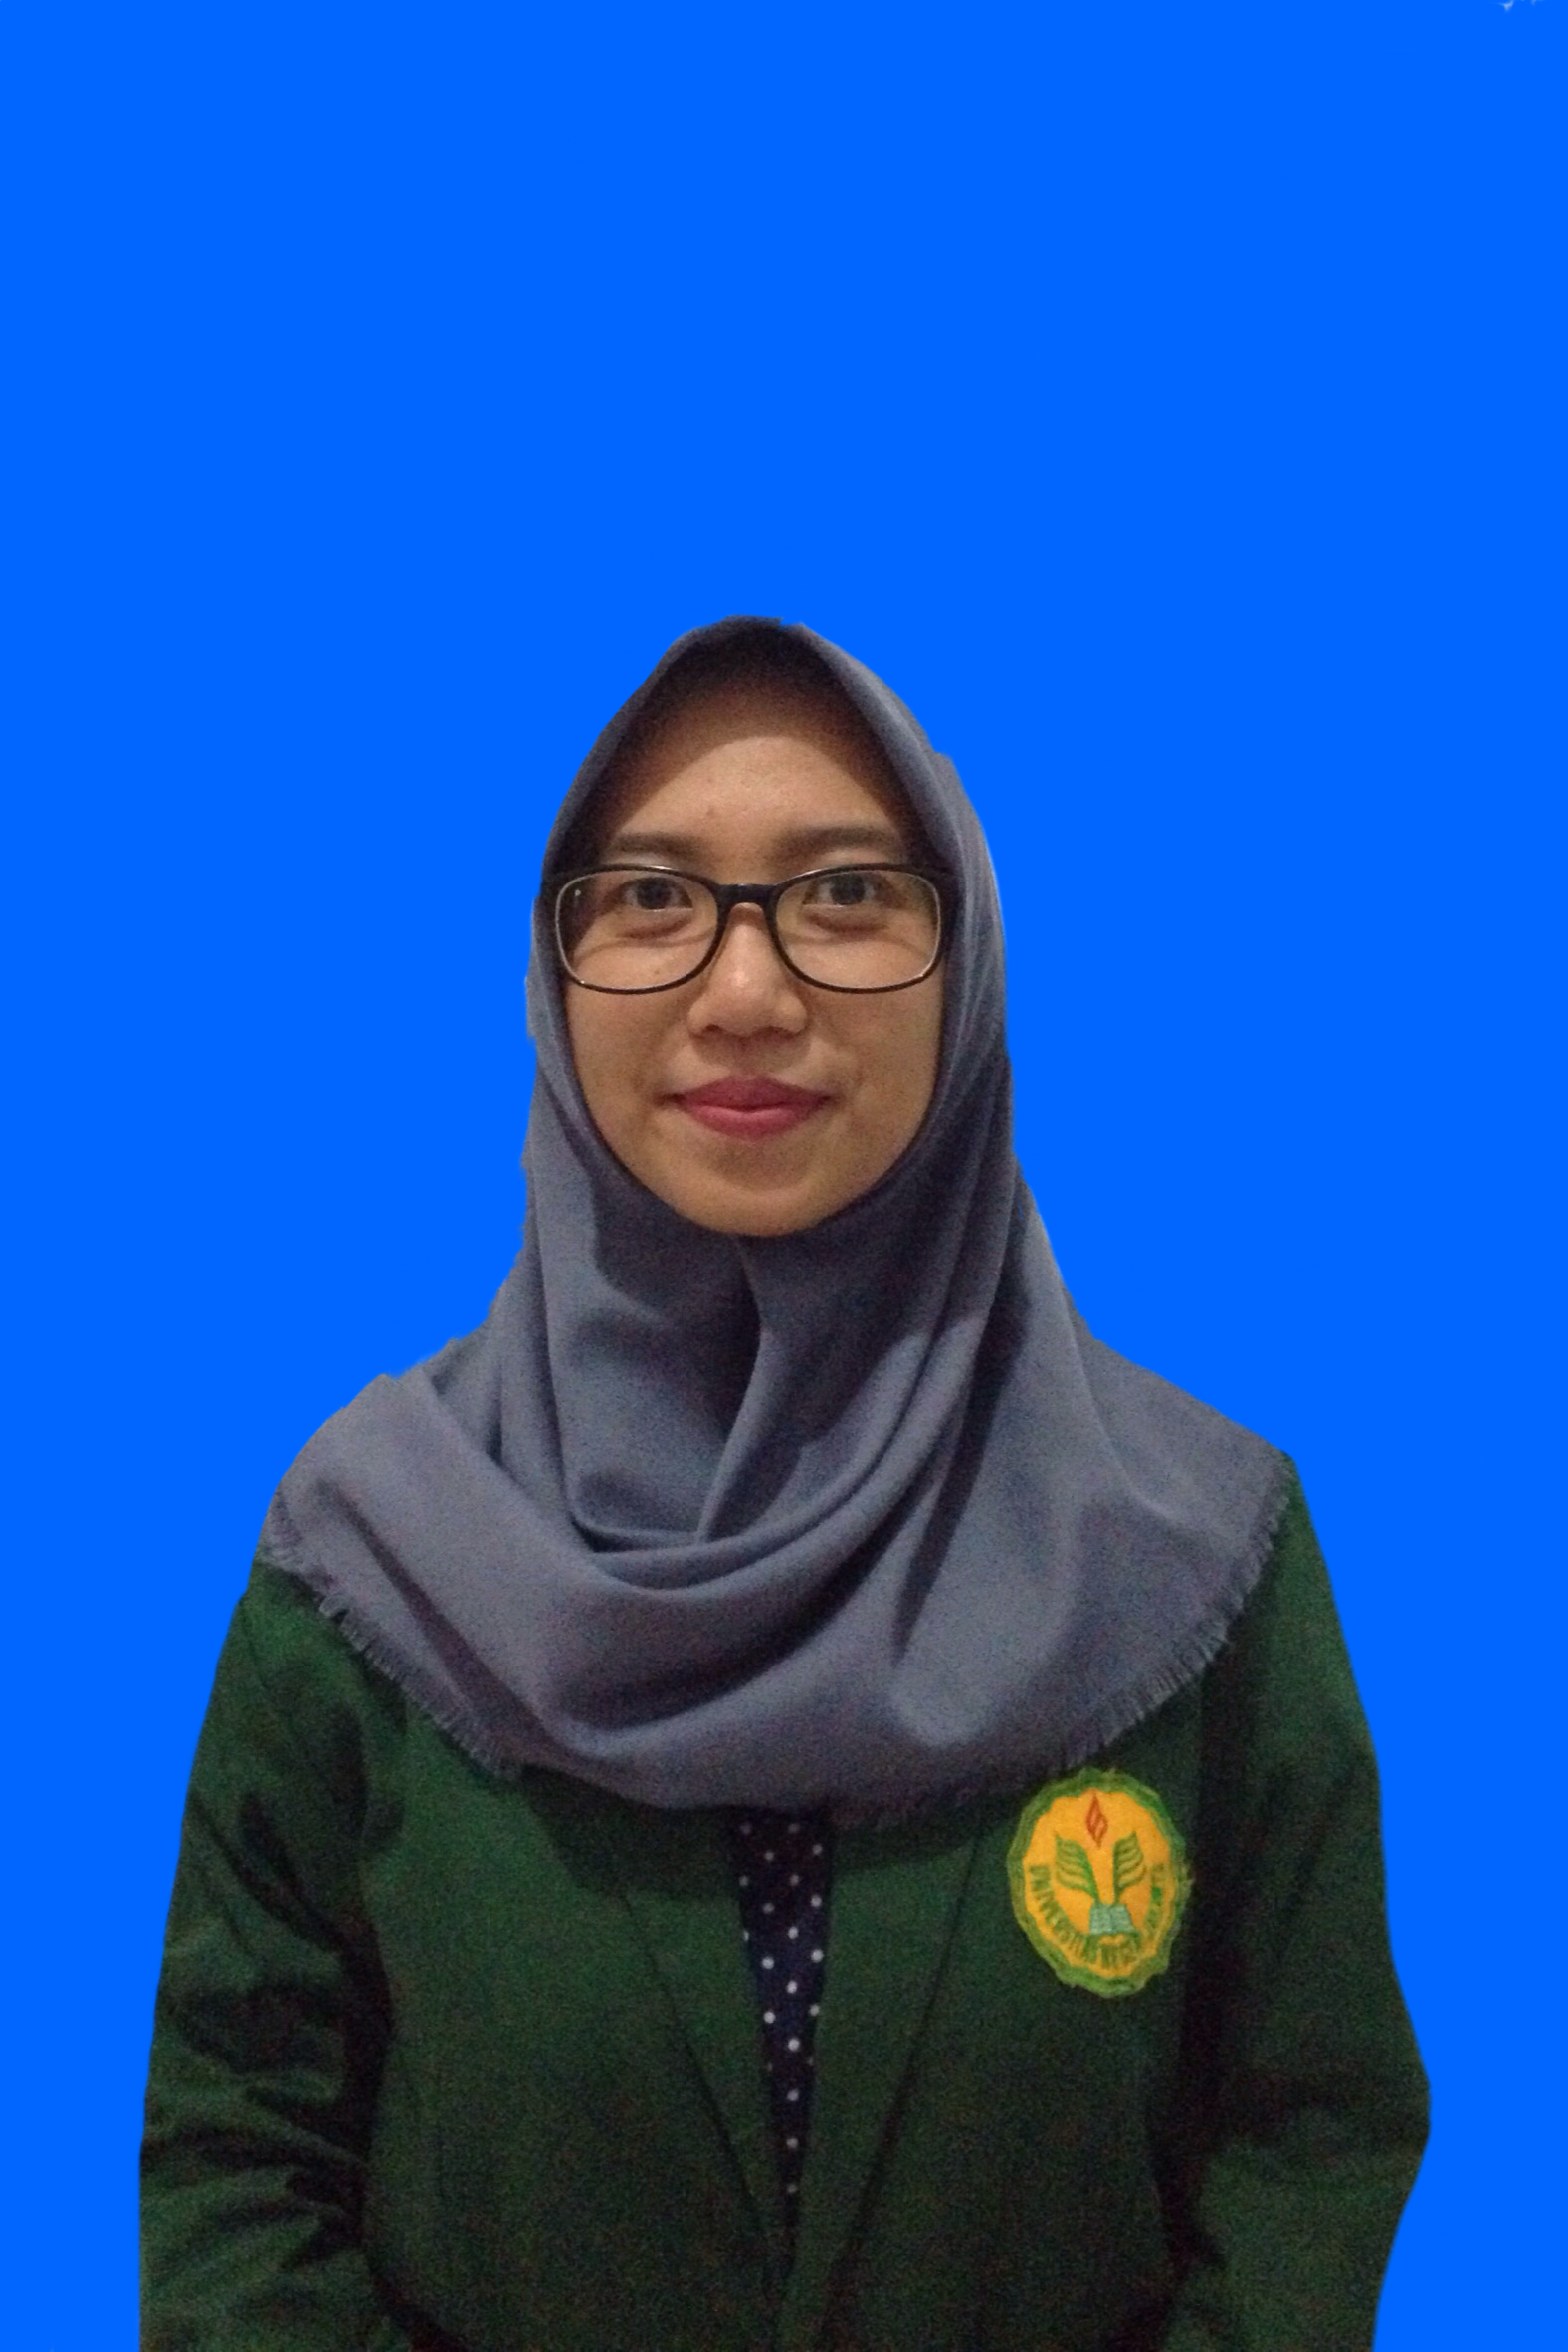
\includegraphics[width=0.4\textwidth]{gambar/matlab/amelia_kalimat}
		\caption{Perbandingan \emph{File} Citra - amelia.bmp}
		\label{amelia_stego}		
	\end{figure}


	Pada Gambar 3.16 dan 3.17 menunjukkan jika dibandingkan secara visual maka tidak tampak perubahan yang terjadi dari \emph{Cover Image} ke \emph{Stego Image}. Tidak tampak perubahan warna ataupun bentuk dari \emph{Cover Image}.

	\subsection{Pengujian Berdasarkan \emph{Fidelity}}
	Pengujian ini berdasarkan proses penyembunyiaan pesan atau \emph{Encoding}. Pada proses penyembunyian pesan dapat berhasil apabila ukuran pesan yang akan disembunyikan sesuai dengan kapasitas \emph{file} citra. Apabila ukuran pesan melebihi kapasitas maksimal dari \emph{file} citra, maka program tidak akan melanjutkan proses \emph{Encoding}. Kapasitas pesan dipengaruhi oleh ukuran \emph{pixel} dari citra \emph{digital}. Semakin besar ukuran \emph{pixel} dari citra \emph{digital}, maka semakin besar pula kapasitas pesan yang bisa disembunyikan.
	
	%masukkin tabel
	\begin{table}[H]
		\centering
		\caption{Karakter Maksimal Pesan pada \emph{File} Citra}
		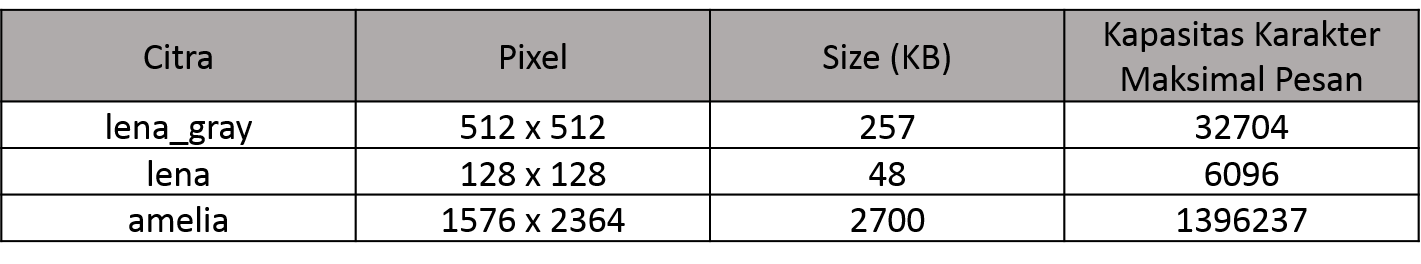
\includegraphics[width=1.0\textwidth]{gambar/table_karaktermax3}
		\label{tabel_karaktermax2}
	\end{table}
	
	Pada Tabel 3.2 terlihat kapasitas karakter maksimal dari ketiga \emph{file} citra. Terlihat bahwa semakin besar ukuran \emph{pixel} dari \emph{file} citra, maka akan semakin besar daya tampung karakternya. Karakter maksimal dari suatu \emph{file} citra dapat dirumuskan dengan:
	
	\begin{center}
	$ charmax = \frac{((height - 1) * width ) * 3}{8}$
	\end{center}

	\begin{table}[H]
		\centering
		\caption{Hasil Proses \emph{Encoding}}
		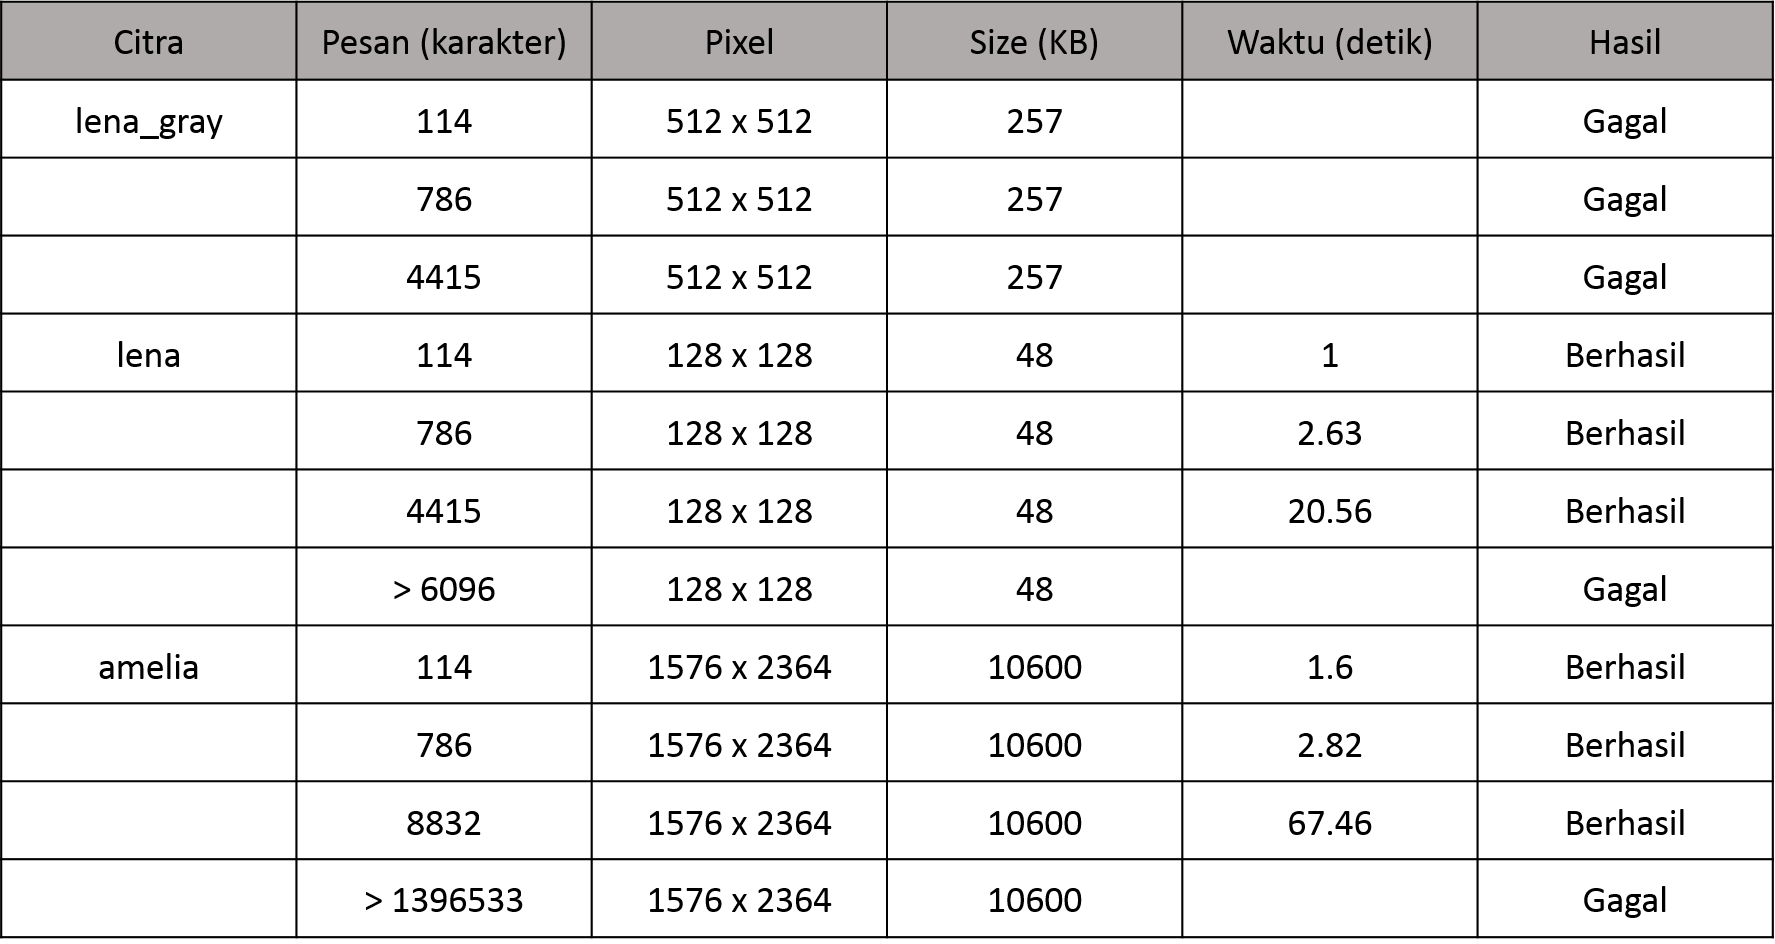
\includegraphics[width=1.0\textwidth]{gambar/table_hasilencode3}
		\label{tabel_hasilencode3}
	\end{table}

	Pada Tabel 3.3 terlihat data \emph{file} citra yang dimasukkan adalah 24 bit dan 32 bit. Setiap  \emph{file} citra dimasukkan pesan atau \emph{Hiddentext} dengan beragam panjang karakter. Panjang dari karakter pesan berpengaruh terhadap kecepatan dalam proses \emph{Encoding}. Semakin panjang karakter yang dimasukkan, maka semakin lama juga waktu yg dibutuhkan. Untuk \emph{file} citra $lena_ gray$ tidak bisa dilakukan proses \emph{Encoding}, karena \emph{file} tersebut adalah \emph{file} 8 bit. Pada \emph{file} citra lena dan amelia, berhasil dilakukan proses \emph{Encoding}, kecuali ketika panjang karakter pesan melebihi kapasitas maksimal dari \emph{file} citra tersebut.

	\subsection{Pengujian Berdasarkan \emph{Recovery}}
	Pengujian ini berdasarkan proses ektraksi pesan atau \emph{Decoding}. Untuk membuktikan apakah program steganografi ini berhasil, maka harus dapat dibuktikan bahwa pesan di dalam \emph{Stego Image} dapat diambil kembali. Jika pengujian dilakukan dengan benar, maka \emph{Hiddentext} dapat ditampilkan sesuai dengan yang dimasukkan. 
	
	Pada penelitian ini, pesan yang dihasilkan dari proses \emph{Decoding} tidak menghasilkan karakter-karakter aneh yang tidak dapat dibaca. Hasil dari pengujian ekstraksi pesan dapat dilihat pada tabel 3.2
	 
	%masukkin tabel
	\begin{table}[H]
		\centering
		\caption{Hasil Proses \emph{Decoding}}
		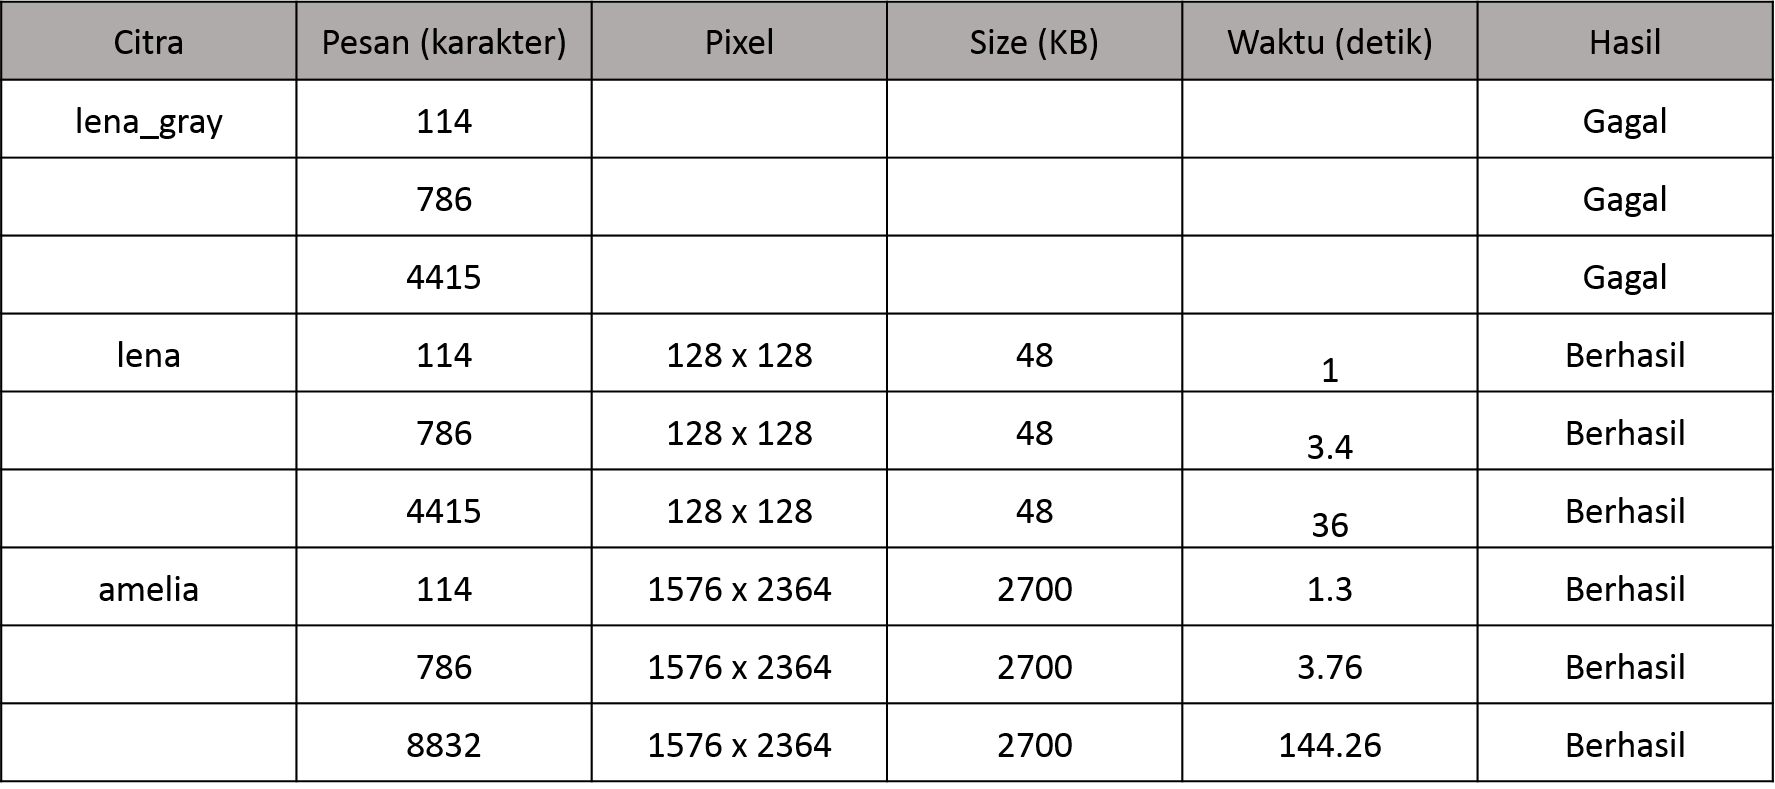
\includegraphics[width=1.0\textwidth]{gambar/table_hasildecode3}
		\label{tabel_hasildecode3}
	\end{table}
	
	Pada proses \emph{Decoding}, besar \emph{pixel} dan ukuran pada \emph{Stego Image}, tidak mengalami perubahan. Hal ini tidak akan memberikan kecurigaan terhadap \emph{file} citra. Waktu yang dibutuhkan dalam proses \emph{Decoding} juga berbanding lurus dengan panjang karakter pesan. Semakin banyak karakter pesan atau \emph{Hiddentext} yang dimasukkan, maka semakin lama waktu yang dibutuhkan. Pada proses \emph{Decoding} terhadap kedua \emph{file} citra hasilnya adalah berhasil. Karena pesan yang ada pada \emph{file} citra tersebut bisa ditampilkan kembali.
	
	Pada pengujian ini juga dilakukan teknik \emph{cropping} pada beberapa \emph{Stego Image}. Setelah dilakukan \emph{cropping}, \emph{Stego Image} tersebut tidak berhasil untuk menampilkan pesan asli yang ada di dalamnya, hanya karakter-karakter aneh yang ditampilkan. 
	
	\begin{table}[H]
		\centering
		\caption{Hasil Proses \emph{Cropping} }
		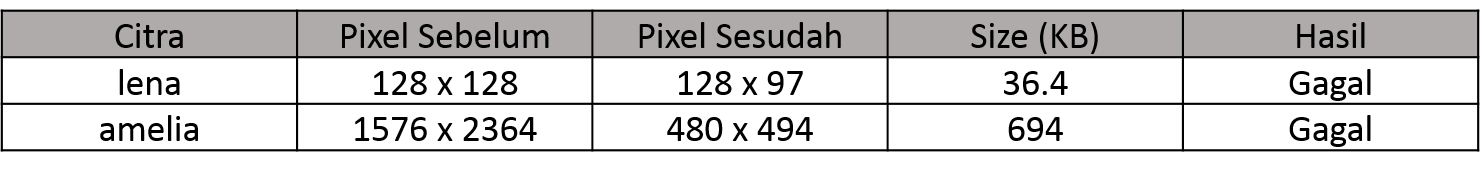
\includegraphics[width=1.0\textwidth]{gambar/table_cropping}
		\label{tabel_cropping}
	\end{table}

	\begin{figure}[H]
		\centering
		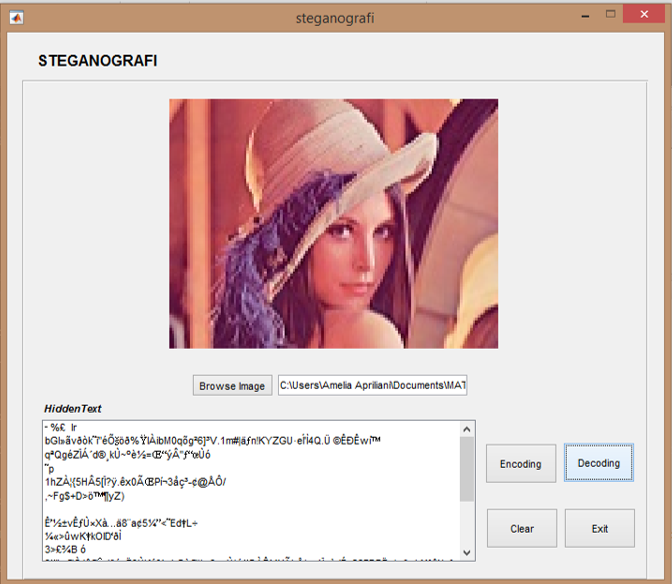
\includegraphics[width=0.7\textwidth]{gambar/matlab/lena_crop}
		\caption{\emph{File} Citra lena.bmp Hasil \emph{Cropping}}
		\label{lena_crop}
	\end{figure}

	\begin{figure}[H]
		\centering
		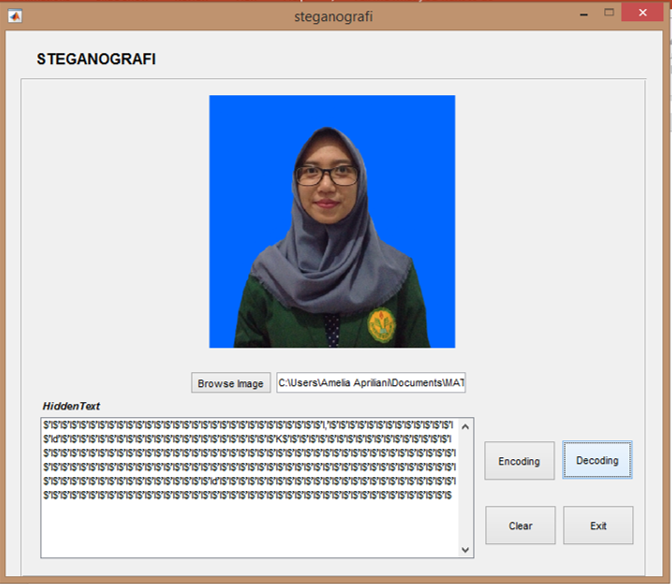
\includegraphics[width=0.7\textwidth]{gambar/matlab/amelia_crop}
		\caption{\emph{File} Citra amelia.bmp Hasil \emph{Cropping}}
		\label{amelia_crop}
	\end{figure}

	Teknik \emph{cropping} dapat menyebabkan \emph{pixel-pixel} pada \emph{file} citra menjadi hilang. Sehingga pesan yang sudah disisipkan di dalam \emph{file} citra tersebut tidak dapat ditampilkan kembali.
		 
	\subsection{Kesimpulan Pengujian}
	Dari pengujian di atas dapat disimpulkan bahwa program steganografi yang dibuat ini menghasilkan hasil yang cukup baik untuk setiap penyembunyian pesan ke dalam \emph{file} citra. Pemilihan \emph{Cover Image} yang akan digunakan dan panjang karakter pesan yang akan dimasukkan sangat berpengaruh, karena semakin besar ukuran \emph{file} citra yang digunakan dan semakin sedikit karakter yang disisipkan pada \emph{file} citra maka semakin sedikit perubahan yang terjadi setelah proses penyisipan pada \emph{file} citra atau kualitas sebelum penyisipan dan setelah penyisipan tidak berpengaruh banyak pada perubahan kualitas citra sebelumnya.
	

%%!TEX root = ./template-skripsi.tex
%-------------------------------------------------------------------------------
%                            	BAB IV
%               		KESIMPULAN DAN SARAN
%-------------------------------------------------------------------------------

\chapter{KESIMPULAN DAN SARAN}

\section{Kesimpulan}
Berdasarkan hasil implementasi dan pengujian program ini, didapat kesimpulan sebagai berikut:

\begin{enumerate}
	\item Format \emph{file} citra yang hanya bisa digunakan adalah format *.bmp 24 bit dan 32 bit.
	
	\item Pesan dalam format teks berhasil untuk disisipkan ke dalam \emph{file} citra dengan metode LSB menggunakan \emph{Software} MATLAB R2016b.
	
	\item \emph{File} citra yang digunakan baik sebelum dan sesudah diproses tidak berubah. Perubahan yang terjadi tidak dapat dilihat secara visual.
	
	\item Pesan dalam \emph{Stego Image} dapat ditampilkan kembali dan sesuai dengan pesan awal.

\end{enumerate}


\section{Saran}
Adapun saran-saran penulis untuk penelitian selanjutnya adalah:
\begin{enumerate}
	\item Program ini hanya dapat menyisipkan pesan berupa teks, diharapkan untuk kedepannya dikembangkan sehingga dapat menyisipkan \emph{file}, gambar atau audio.
	
	\item Media yang digunakan berupa \emph{file} citra, diharapkan dapat menggunakan media lain seperti audio.
	
	\item Program steganografi ini masih dikembangkan dengan MATLAB untuk perangkat komputer, diharapkan dapat dikembangkan lebih lanjut untuk perangkat \emph{mobile}. 
	
\end{enumerate}


% Baris ini digunakan untuk membantu dalam melakukan sitasi
% Karena diapit dengan comment, maka baris ini akan diabaikan
% oleh compiler LaTeX.
\begin{comment}
\bibliography{daftar-pustaka}
\end{comment}

%%!TEX root = ./template-skripsi.tex
%-------------------------------------------------------------------------------
%                            	BAB V
%               		KESIMPULAN DAN SARAN
%-------------------------------------------------------------------------------

\chapter{KESIMPULAN DAN SARAN}

\section{Kesimpulan}
	Berdasarkan hasil implementasi dan pengujian konten, tampilan, serta fungsionalitas aplikasi ini, didapat kesimpulan sebagai berikut:

	\begin{enumerate}
		\item Bentuk aplikasi kumpulan resep masakan terintegrasi \textit{food channel} YouTube dapat dilihat pada Gambar \ref{mock-welcome} - Gambar \ref{mock-feedback}. Bentuk spesifik dimana \textit{food channel} YouTube diletakkan pada aplikasi tersebut terdapat pada Gambar \ref{detail_bahan} dan Gambar \ref{detail_cara}.
		
		\item Aplikasi kumpulan resep masakan terintegrasi \textit{food channel} YouTube dikembangkan dengan mengacu pada \textit{System Development Life Cycle} (SDLC) model Spiral dengan tahapan yaitu Identifikasi, Desain, Konstrusi dan Pembangunan, dan yang terakhir adalah Evaluasi.
		
		\item YouTube dapat diintegrasikan dengan aplikasi Android dengan menggunakan YouTube Android Player API. Penggunaan API YouTube tersebut disesuaikan dengan kebutuhannya dalam sebuah antarmuka aplikasi Android. Apabila digunakan pada Activity utuh maka dapat digunakan YouTubePlayerView. Sedangkan jika menggunakan Activity yang terdiri dari satu atau lebih Fragment, maka digunakan YouTubePlayerFragment. 

		\item Berdasarkan hasil uji coba, dapat disimpulkan bahwa \textit{food channel} YouTube berhasil diimplementasikan pada aplikasi yang dikembangkan oleh penulis. Hal tersebut ditunjukkan dengan item penilaian video YouTube dapat dimainkan dengan baik juga menempati peringkat teratas dalam segi tampilan serta video YouTube yang diputar sesuai dengan resepnya, menempati peringkat teratas dalam proses uji coba dari segi konten. Fitur-fitur lainnya turut melengkapi aplikasi resep masakan terintegrasi \textit{food channel} YouTube ini. Dengan kata lain, aplikasi ini berhasil diuji dengan baik dan siap dirilis ke masyarakat luas. 
	\end{enumerate}


\section{Saran}
	Adapun saran-saran penulis untuk penelitian selanjutnya adalah:
	\begin{enumerate}
		\item Menambahkan informasi bagaimana cara memasak yang baik dan benar sesuai dengan standar yang berlaku dalam dunia memasak serta menambah kosakata bahasa asing maupun bahasa daerah untuk memperkaya pengetahuan pengguna aplikasi. 
		
		\item Menambah kapasitas \textit{wishlist} menjadi lebih dari 3.
		
		\item Membuat aplikasi yang dapat menjangkau lebih banyak versi Android, termasuk versi Android sebelum API 21 atau Android 5.0 (Lollipop). 
		
		\item Membuat aplikasi kumpulan resep masakan yang mampu memuat lebih dari satu video pada setiap resepnya.
		
		\item Menggunakan basis data Firebase sebagai pengganti SQL karena Firebase juga merupakan produk Google sama dengan Android. Banyak kemampuan yang mampu dimaksimalkan dengan penggunaan Firebase sebagai basis data dari sebuah aplikasi Android.
		
		\item Jika masih mengembangkan dengan menggunakan CodeIgniter-Based API ataupun API berbasis \textit{web framework} lainnya, penggunaan Retrofit menggantikan Volley sangat disarankan karena kecepatan akses data yang jauh lebih cepat daripada Volley. 

	\end{enumerate}

	
% Baris ini digunakan untuk membantu dalam melakukan sitasi
% Karena diapit dengan comment, maka baris ini akan diabaikan
% oleh compiler LaTeX.
\begin{comment}
\bibliography{daftar-pustaka}
\end{comment}

%-----------------------------------------------------------------
%Disini akhir masukan Bab
%-----------------------------------------------------------------


%-----------------------------------------------------------------
% Disini awal masukan untuk Daftar Pustaka
% - Daftar pustaka diambil dari file .bib yang ada pada folder ini
%   juga.
% - Untuk memudahkan dalam memanajemen dan menggenerate file .bib
%   gunakan reference manager seperti Mendeley, Zotero, EndNote,
%   dll.
%-----------------------------------------------------------------
%\bibliography{IEEEabrv,daftar-pustaka}
\begin{thebibliography}{99}
	\bibitem{adiria}Adiria. (2010). "ANALISIS DAN PERANCANGAN APLIKASI STEGANOGRAFI PADA CITRA DIGITAL DENGAN MENGGUNAKAN METODE LSB (LEAST SIGNIFICANT BIT)". Skripsi Sarjana pada Universitas Islam Negeri Jakarta
	
	\bibitem{arymurthy}Arymurthy, A. M., dan Setiawan, S. (1992). "Pengantar Pengolahan Citra. Jakarta: PT Elex Media Komputindo".
	
	\bibitem{ascii} ASCII Table.  2010. "ASCII Table and Description".  ASCII Table [Online]. Tersedia: \url{https://www.asciitable.com}. [17 April 2018].
	
	\bibitem{bunyamin}Bunyamin, H., dan Adrian. (2009). "Aplikasi Steganography pada File dengan Menggunakan Teknik Low Bit Encoding dan Least Significant Bit". Jurnal Informatika UKM, Vol. 5, No. 2, pp. 107–117.
	
	\bibitem{elgabar}Elgabar, Eltyeb E. A bed. (2013). "Comparison of LSB Steganography in BMP and JPEG Images". International Journal of Soft Computing and Engineering (IJSCE), ISSN: 2231-2307, Vol.3, Issue-5.
	
	\bibitem{elgabar2}Elgabar, Eltyeb E. A bed dan Mohammed, Fakhreldeen A. (2013). "JPEG versus GIF Images in forms of LSB Steganography".  International Journal of Computer Science and Network (IJCSN), Vol. 2, Issue 6.
	
	\bibitem{gautam}Gautama, Prakriti dan Sharma, Deepak. (2015). "A Survey on Digital Image Steganography Techniques". International Journal of Electronics, Electrical and Computational System (IJEECS), ISSN 2348-117X, Vol. 4, Issue 11. 
	
	\bibitem{hermawati}Hermawati, F. A. (2013). "Pengolahan Citra Digital". Yogyakarta: ANDI.
	
	\bibitem{irfan}Irfan. (2013). "Penyembunyian Informasi (steganography) Gambar Menggunakan Metode LSB (Least Significant Bit)". Rekayasa Teknologi Vol. 5, No. 1.
	
	\bibitem{joshi}Joshi, K., dan Yadav, R. (2015). "A New LSB-S Image Steganography Method Blend with Cryptography for Secret Communication". Third International Conference on Image Infomation Processing.
	
	\bibitem{kessler}Kessler, G. C. (2001). "Steganography Hiding Data Within Data".
	
	\bibitem{kadam}M. K., Kadam, K., Koshti, A., dan Dunghav, P. (2012). "Steganography Using Least Signicant Bit Algorithm". International Journal of Engineering Research and Applications (IJERA), Vol. 2, Issue 3, pp. 338-341.
	
	\bibitem{munir04}Munir, R. (2004). "Pengolahan Citra Digital". Bandung: Informatika.
	
	\bibitem{munir}Munir, R. (2006). "Kriptografi". Bandung: Informatika.
	
	\bibitem{pakereng}Pakereng, M.A Ineke, Beeh, Yos Richard, dan Endrawan, Sonny. (2010). "Perbandingan Steganografi Metode Spread Spectrum dan Least Significant Bit (LSB) Antara Waktu Proses dan Ukuran File Gambar". JURNAL INFORMATIKA, VOL. 6 NO. 1.
	
	\bibitem{pavani}M., Pavani, S., Naganjaneyulu, dan C., Nagaraju. (2013). "A Survey on LSB Based Steganography Methods". International Journal Of Engineering And Computer Science, Vol. 2, Issue pp. 2464-2467.
	
	\bibitem{prasetyo}Prasetyo, F. P. (2010). "STEGANOGRAFI MENGGUNAKAN METODE LSB DENGAN SOFTWARE MATLAB". Skripsi Sarjana pada Universitas Islam Negeri Jakarta
	
	\bibitem{prayudi}Prayudi, Y., dan Kuncoro, P. S. (2005). "IMPLEMENTASI STEGANOGRAFI MENGGUNAKAN TEKNIK ADAPTIVE MINIMUM ERROR LEAST SIGNIFICANT BIT REPLACEMENT (AMELSBR)". Seminar Nasional Aplikasi Teknologi Informasi.
	
	\bibitem{rakhmat}Rakhmat, B., dan Fairuzabadi, M. (2010). "STEGANOGRAFI MENGGUNAKAN METODE LEAST SIGNIFICANT BIT DENGAN KOMBINASI ALGORITMA KRIPTOGRAFI VIGENÈRE DAN RC4". Jurnal Dinamika Informatika, Volume 5, Nomor 2.
	
	\bibitem{setiana}Setiana, dan Mahmudy, W. F. (2006). "Steganografi Pada File Citra Bitmap 24 Bit Untuk Pengamanan Data Menggunakan Metode Least Significant Bit (LSB) Insertion". Kursor, vol. 2, no. 2, pp. 38-44.
	
	\bibitem{wikipedia1}Wikipedia. (n.d.). Retrieved from https://id.wikipedia.org/wiki/Steganografi
		
		
	
\end{thebibliography}
\addcontentsline{toc}{chapter}{DAFTAR PUSTAKA}
%-----------------------------------------------------------------
%Disini akhir masukan Daftar Pustaka
%-----------------------------------------------------------------

%\addcontentsline{toc}{chapter}{LAMPIRAN}
\appendix 
\chapter{\emph{Source Code}}
	\begin{verbatim}
		char_max = (row -1)*(column);
		char_max = round((char_max*3)/8);
		
		%Cek Kondisi Lokasi
		lokasi = get(handles.kolom_lokasi, 'String')
		if isempty(lokasi) 
		msgbox('Gambar belum dimasukkan','Peringatan','warn');
		return;    
		end		
	
		%Cek Kondisi Kolom Hiddentext
		hiddentext = get(handles.edit_pesan,'String');
		if isempty(hiddentext)
			msgbox('Pesan belum dimasukkan','Peringatan','warn');
		return;    
		end
	
		%Menghitung Panjang Pesan
		row_max = row;
		column_max = column;
		hiddentext_length = length(hiddentext) 
		if hiddentext_length < char_max 
		hiddentext_biner = strcat(reshape(dec2bin(double(hiddentext),8).',1,[]), '00000000')
		hiddentext_save = hiddentext_biner;
		hiddentext_asli = char(bin2dec(reshape(hiddentext_biner,8,[]).')).'
		
		else
		msgbox('Maaf,pesan terlalu panjang','peringatan','warn');
		return;
		end
	
		%Encoding
		hiddentext_length = hiddentext_length*8;
		for i = 1:row_max-1
		for j = 1:column_max    
		if hiddentext_length ~= 0
		image_biner_red = dec2bin(image_red(i,j),8);
		image_biner_red(1,8) = hiddentext_biner(1,1);
		image_red(i,j) = bin2dec(image_biner_red); 
		
		hiddentext_biner(1:1) = [];  
		hiddentext_length = length(hiddentext_biner);            
		end
		
		if hiddentext_length ~= 0
		image_biner_green = dec2bin(image_green(i,j),8);
		image_biner_green(1,8) = hiddentext_biner(1,1);
		image_green(i,j) = bin2dec(image_biner_green);
		
		hiddentext_biner(1:1) = []; 
		hiddentext_length = length(hiddentext_biner); 
		end
		
		if hiddentext_length ~= 0
		image_biner_blue = dec2bin(image_blue(i,j),8);
		image_biner_blue(1,8) = hiddentext_biner(1,1); 
		image_blue(i,j) = bin2dec(image_biner_blue); 
		
		hiddentext_biner(1:1) = []; 
		hiddentext_length = length(hiddentext_biner); 
		end
		end
		end
		
		stego_image(:,:,1) = uint8(image_red);
		stego_image(:,:,2) = uint8(image_green);
		stego_image(:,:,3) = uint8(image_blue);
		
		[nama_file, direktori] = uiputfile('*.bmp','Simpan Stego Image');
		if direktori == 0
		return;
		end
		nama = fullfile(direktori, nama_file);
		imwrite(stego_image, nama, 'bmp');
		msgbox('Stego Image telah berhasil dibuat','pemberitahuan');	
	
		%Decoding
		hiddentext = '';
		var_null = 1;
		for i = 1:row_max-1
		for j = 1:column_max
		biner_length = length(hiddentext);
		if biner_length < hiddentext_length && var_null<=8
		image_biner_red = dec2bin(image_red(i,j),8); 
		hiddentext_red = image_biner_red(1,8);
		hiddentext = strcat(hiddentext, hiddentext_red);
		if hiddentext_red == 0
		var_null = var_null + 1;
		else
		var_null = 1;
		end   
		else
		hiddentext_asli = char(bin2dec(reshape(hiddentext,8,[]).')).';
		set(handles.edit_pesan,'String',hiddentext_asli);
		return;
		end
		
		biner_length = length(hiddentext);
		if biner_length < hiddentext_length && var_null<=8
		image_biner_green = dec2bin(image_green(i,j),8);
		hiddentext_green = image_biner_green(1,8);
		hiddentext = strcat(hiddentext, hiddentext_green);
		if hiddentext_green == 0
		var_null = var_null+1;
		else
		var_null = 1;
		end   
		else
		hiddentext_asli = char(bin2dec(reshape(hiddentext,8,[]).')).';
		set(handles.edit_pesan,'String',hiddentext_asli);
		return;
		end
		
		biner_length = length(hiddentext);
		if biner_length < hiddentext_length && var_null<=8
		image_biner_blue = dec2bin(image_blue(i,j),8);
		hiddentext_blue = image_biner_blue(1,8);
		hiddentext = strcat(hiddentext, hiddentext_blue);
		if hiddentext_blue == 0
		var_null = var_null+1;
		else
		var_null = 1;
		end   
		else
		hiddentext_asli = char(bin2dec(reshape(hiddentext,8,[]).')).';
		set(handles.edit_pesan,'String',hiddentext_asli);
		return;
		end
		
		end
		end
	\end{verbatim}


%\pagestyle{empty}
\chapter*{\centering \large DAFTAR RIWAYAT HIDUP}
\thispagestyle{empty}

\begin{wrapfigure}{l}{4cm}
	\vspace{-25pt}
	\begin{center}
		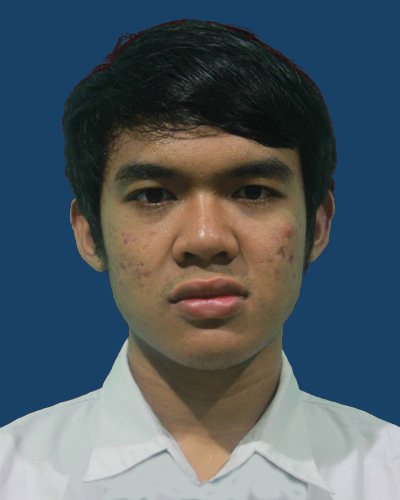
\includegraphics[width=0.27\textwidth]{gambar/pas-foto}
	\end{center}
	\vspace{-80pt}
\end{wrapfigure}

\noindent \textbf{AMELIA APRILIANI.}  Lahir di Jakarta, 23 April 1996.  Anak pertama dari pasangan Bapak H. Nurdin dan Ibu Nurjanah. Saat ini beralamatkan di Jl. Olah Raga I RT.010 RW.05 No.64, Cililitan Jakarta Timur.

\vspace{0.5cm}
\noindent
\begin{center}
	\begin{flushright}
		\begin{tabular}{lcl}
			No. Ponsel	& :&  085776210885 \\
			Email	& :&  ameliaapriliani85@gmail.com
		\end{tabular}
	\end{flushright}
\end{center}
\vspace{0.5cm}

\noindent \textbf{Riwayat Pendidikan} : Penulis mengawali pendidikan di TK As-Saadah pada tahun 2001 - 2002, dan kemudian melanjutkan pendidikan di SDN Cililitan 01 Pagi pada tahun 2002 - 2008. Setelah itu, penulis melanjutkan ke SMPN 150 Jakarta hingga tahun 2011. Kemudian melanjutkan ke SMAN 14 Jakarta pada tahun 2011-2014. Di Tahun 2014 penulis melanjutkan ke Universitas Negeri Jakarta (UNJ), Program Studi Ilmu Komputer, melalui jalur PENMABA. Di akhir tahun 2018 (Kamis, 09 Agustus 2018) penulis telah memperoleh gelar Sarjana Komputer (S.Kom), Program Studi Ilmu Komputer, Fakultas Matematika dan Ilmu Pengetahuan Alam, Universitas Negeri Jakarta.

\noindent \textbf{Riwayat Organisasi} : Selama di bangku perkuliahan, penulis aktif di organisasi keilmiahan Program Studi Ilmu Komputer sebagai anggota merangkap Sekertaris periode 2015-2016. Penulis juga berpartisipasi dalam kegiatan BINER (Be Innovative and Educated Researcher) yaitu kegiatan workshop dan seminar yang diadakan oleh DEFAULT, dimana penulis tergabung sebagai anggota merangkap Sekertaris. 

\end{document}